% In questo file vengono definiti comandi (macro) utili in tutti i documenti

\newcommand{\gruppo}{\textit{Sirius}} % nome gruppo
\newcommand{\progetto}{\textit{Sequenziatore}} % nome progetto
\newcommand{\capitolato}{\href{http://www.math.unipd.it/~tullio/IS-1/2013/Progetto/C4p.pdf}{http://www.math.unipd.it/~tullio/IS-1/2013/Progetto/C4p.pdf}} 

% GLOSSARIO
\newcommand{\lastversionG}{4.0.0}
\newcommand{\Glossario}{\textit{Glossario\_{}v\lastversionG{}.pdf}}
\newcommand{\doctitleG}{Glossario}
\newcommand{\infoG}{\doctitleG\ v\lastversionG}

% NORME DI PROGETTO
\newcommand{\lastversionNDP}{4.0.0}
\newcommand{\NormeDiProgetto}{\textit{NormeDiProgetto\_{}v\lastversionNDP{}.pdf}}
\newcommand{\doctitleNDP}{Norme di progetto}
\newcommand{\infoNDP}{\doctitleNDP\ v\lastversionNDP}

% ANALISI DEI REQUISITI
\newcommand{\lastversionAR}{3.0.0}
\newcommand{\AnalisiDeiRequisiti}{\textit{AnalisiDeiRequisiti\_{}v\lastversionAR{}.pdf}}
\newcommand{\doctitleAR}{Analisi dei requisiti}
\newcommand{\infoAR}{\doctitleAR\ v\lastversionAR}

% Studio di fattibilita
\newcommand{\lastversionSDF}{2.0.0}
\newcommand{\StudioDiFattibilita}{\textit{StudioDiFattibilita\_{}v\lastversionSDF{}.pdf}}
\newcommand{\doctitleSDF}{Studio Di Fattibilità}
\newcommand{\infoSDF}{\doctitleSDF\ v\lastversionSDF}

% Piano di qualifica
\newcommand{\lastversionPDQ}{4.0.0}
\newcommand{\PianoDiQualifica}{\textit{PianoDiQualifica\_{}v\lastversionPDQ{}.pdf}}
\newcommand{\doctitlePDQ}{Piano Di Qualifica}
\newcommand{\infoPDQ}{\doctitlePDQ\ v\lastversionPDQ}

% VERBALE 2014-02-03
\newcommand{\lastversionVb}{2.0.0}
\newcommand{\VerbaleB}{\textit{Verbale2014-02-03\_{}v\lastversionVb{}.pdf}}
\newcommand{\doctitleVb}{Verbale 2014-02-03}
\newcommand{\infoVb}{\doctitleVb\ v\lastversionVb}

% VERBALE 2014-07-20
\newcommand{\lastversionVN}{1.0.0}
\newcommand{\VerbaleN}{\textit{Verbale2014-07-20\_{}v\lastversionVN{}.pdf}}
\newcommand{\doctitleVN}{Verbale 2014-07-20}
\newcommand{\infoVN}{\doctitleVN\ v\lastversionVN}

%Piano di progetto
\newcommand{\lastversionPDP}{4.0.0}
\newcommand{\PianoDiProgetto}{\textit{PianoDiProgetto\_{}v\lastversionPDP{}.pdf}}
\newcommand{\doctitlePDP}{Piano Di Progetto}
\newcommand{\infoPDP}{\doctitlePDP\ v\lastversionPDP}
%Specifica Tecnica
\newcommand{\lastversionST}{3.0.0}
\newcommand{\SpecificaTecnica}{\textit{SpecificaTecnica\_{}v\lastversionST{}.pdf}}
\newcommand{\doctitleST}{Specifica Tecnica}
\newcommand{\infoST}{\doctitleST\ v\lastversionST}
%Definizione di prodotto
\newcommand{\lastversionDP}{2.0.0}
\newcommand{\DefinizioneDiProdotto}{\textit{DefinizioneDiProdotto\_{}v\lastversionDP{}.pdf}}
\newcommand{\doctitleDP}{Definizione Di Prodotto}
\newcommand{\infoDP}{\doctitleDP\ v\lastversionDP}

% MANUALE UTENTE
\newcommand{\lastversionMU}{2.0.0}
\newcommand{\ManualeUtente}{\textit{ManualeUtente\_{}v\lastversionMU{}.pdf}}
\newcommand{\doctitleMU}{Manuale utente}
\newcommand{\infoMU}{\doctitleMU\ v\lastversionMU}

% MANUALE PROCESS OWNER
\newcommand{\lastversionMPO}{2.0.0}
\newcommand{\ManualePO}{\textit{ManualeProcessOwner\_{}v\lastversionMPO{}.pdf}}
\newcommand{\doctitleMPO}{Manuale process owner}
\newcommand{\infoMPO}{\doctitleMPO\ v\lastversionMPO}% macro
\newcommand{\lastversion}{1.0.0}%versione del documento
\newcommand{\doctitle}{Definizione di prodotto}%nome documento
\newcommand{\info}{\doctitle\ v\lastversion}
\documentclass[11pt,a4paper]{article}
\usepackage[a4paper,portrait,top=3.5cm,bottom=3.5cm,left=3cm,right=3cm,bindingoffset=5mm]{geometry}


\usepackage[italian]{babel}
\usepackage{ucs} %unicode sistema gli accenti
\usepackage[utf8x]{inputenc} %unicode sistema gli accenti
\usepackage{fancyhdr}
\usepackage{subfigure} % per figure affiancate
\usepackage{hyperref}
\usepackage{float} % per far bene le figures
\usepackage{indentfirst}
\usepackage{longtable}
\usepackage{color}
\usepackage{colortbl}
\usepackage{rotating}
\usepackage[table]{xcolor}
\usepackage{wrapfig}
\usepackage{array}
\usepackage{eurosym}
\usepackage{graphicx}
\usepackage{breakurl}
\usepackage{lastpage} % total page count
\usepackage{chngpage}
\usepackage{amsfonts}
\usepackage{listings}
\usepackage{bookmark} % custom bookmarks

%\graphicspath{{./Pics}} % cartella di salvataggio immagini

% Per l'indice analitico
%\usepackage{makeidx}
%\makeindex

%pagestyle{fancy}
%\renewcommand{\chaptermark}[1]{\markboth{\thechapter.\ #1}{}}
%\renewcommand{\sectionmark}[1]{\markright{\thesection.\ \ #1}{}}
%\fancyhead{}
%comandi dell header
%\fancyhead[EL]{\slshape \leftmark}
%\fancyhead[OR]{\slshape \rightmark}
%\fancyfoot[EC,OC]{\slshape \thepage}

\pagestyle{fancy}
%\newcommand{\license}{\href{http://creativecommons.org/licenses/by/3.0/}{Some rights reserved}}
\newcommand{\groupname}{Sirius - Sequenziatore}

\newcommand{\subscript}[1]{\raisebox{-0.6ex}{\scriptsize #1}}
%\newcommand{\subscript}[1]{\ensuremath{_{\textrm{#1}}}}
%\renewcommand{\sectionmark}[1]{\markright{\thesection.\ #1}}
%\lhead{\nouppercase{\rightmark}}
%\rhead{\nouppercase{\leftmark}}
%\renewcommand{\chaptermark}[1]{\markboth{\thechapter.\ #1}{}}


\fancypagestyle{plain}{%
	\chead{}
	\lfoot{\info}
	\cfoot{}
	\rfoot{\thepage\ / \pageref{LastPage}}
	\renewcommand{\headrulewidth}{0.3pt}
	\renewcommand{\footrulewidth}{0.3pt}
}
	\lhead{\setlength{\unitlength}{1mm}
        \begin{picture}(0,0)
                \put(5,0){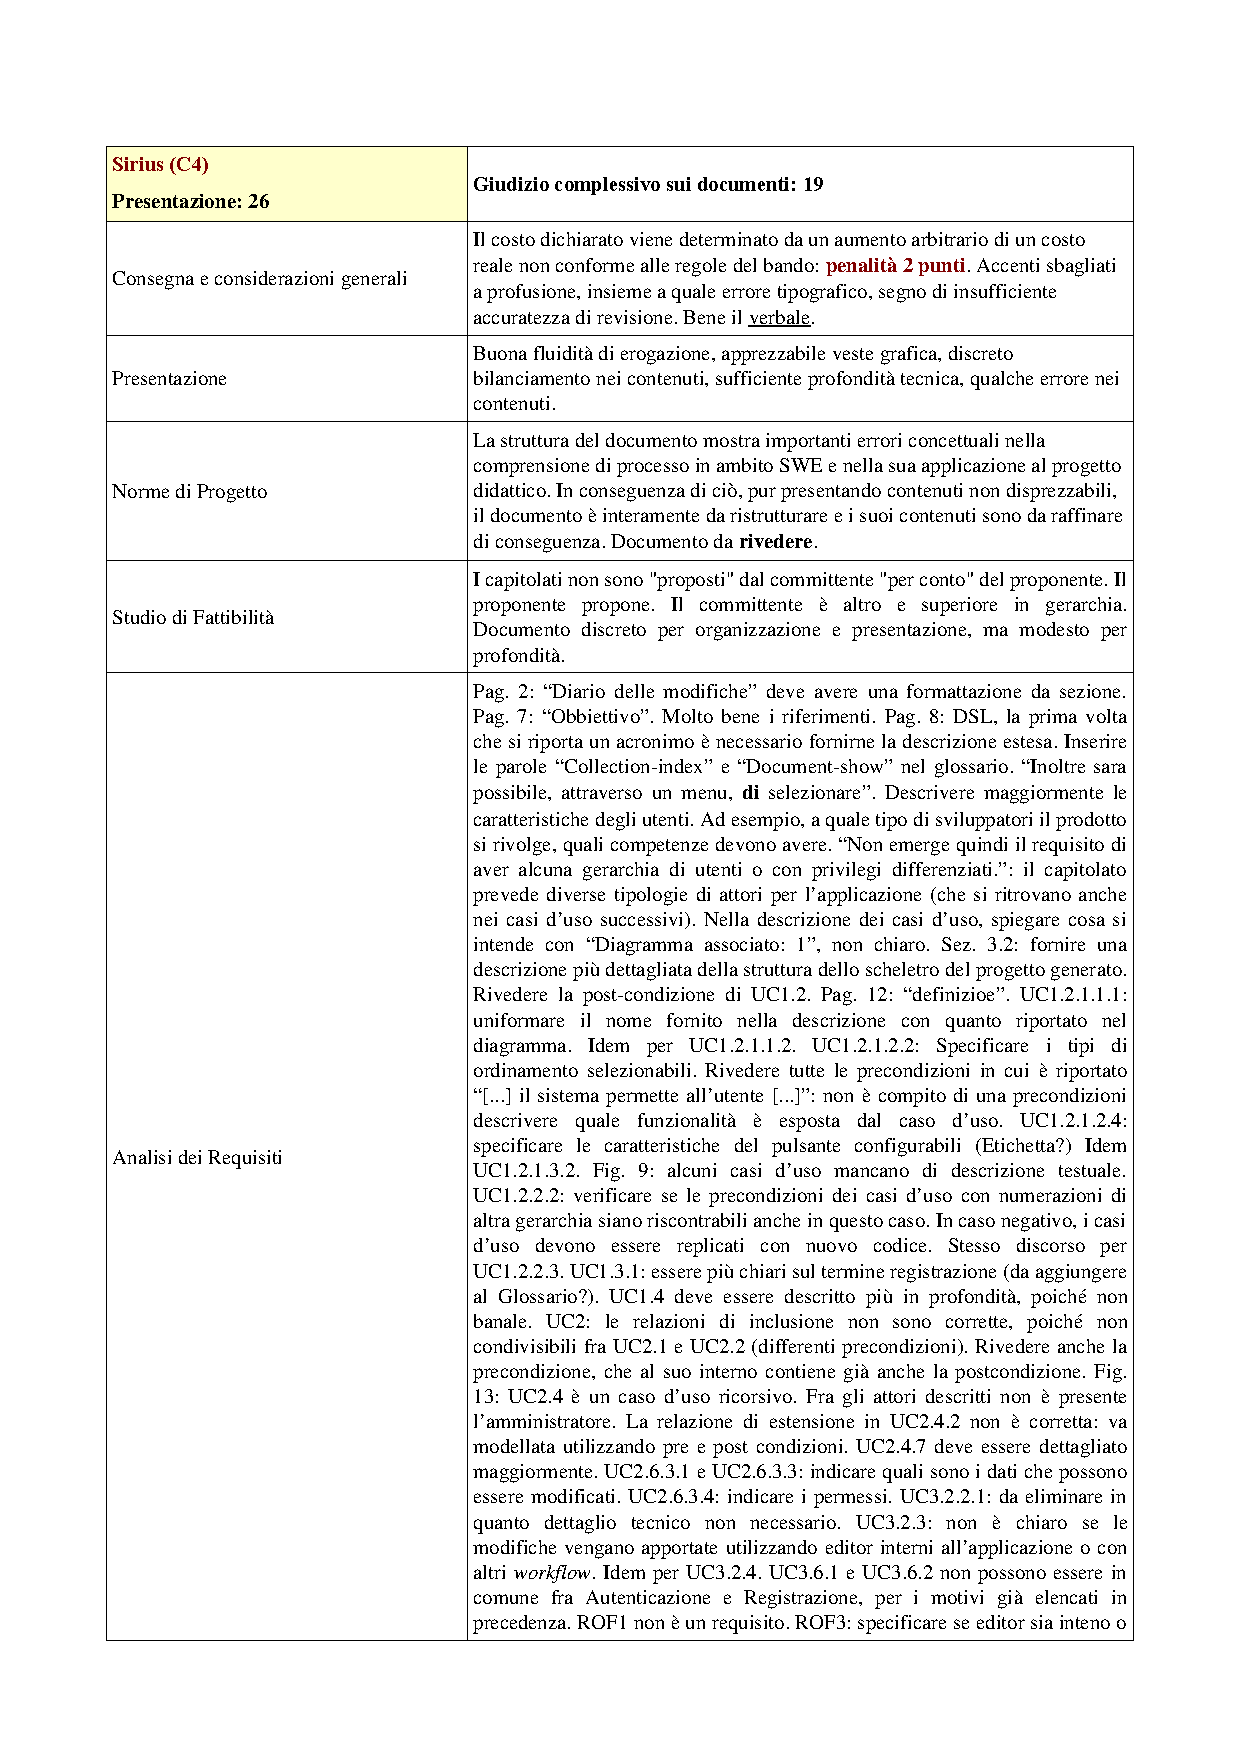
\includegraphics[scale=0.001]{img/Sirius.png}}
        \end{picture}}
	\rhead{\groupname}
	\chead{}
	\lfoot{\info}
	\cfoot{}
%	\rfoot{\thepage}
	\rfoot{\thepage\ / \pageref{LastPage}}
	\renewcommand{\headrulewidth}{0.3pt}
	\renewcommand{\footrulewidth}{0.3pt}
\linespread{1.2}	% valore interlinea


\fancypagestyle{romano}{
	\lhead{\setlength{\unitlength}{1mm}
        \begin{picture}(0,0)
                \put(5,0){
\includegraphics[scale=0.03]{../modello/img/sirius.png}}
        \end{picture}}
	\chead{}
	\rhead{\groupname}
	\lfoot{\info}
	\cfoot{}
	\rfoot{\thepage}
	\renewcommand{\headrulewidth}{0.3pt}
	\renewcommand{\footrulewidth}{0.3pt}
}



\hypersetup{
    colorlinks=true,linkcolor=[rgb]{0.11,0.55,0.83
    },          % colore link interni
    urlcolor=cyan           %colore link esterni
}
\definecolor{err}{rgb}{0.9,0.1,0.1}
\definecolor{rt}{rgb}{0.1,0.6,0.8}
\definecolor{grey}{rgb}{0.4,0.3,0.4}
\definecolor{mycolor}{rgb}{0.67,1,0.18}

\bibliographystyle{plain_ita}%bibliografia stile italiano

\pagenumbering{Roman}
\setlength\parindent{0pt} % sempre senza indentatura
% fine layout% layout

\makeatletter
\renewcommand*{\BreakableSlash}{%
  \leavevmode
  \prw@zbreak
  %
  \discretionary{-}{}{}%
  \prw@zbreak
}

\tolerance 1414
\hbadness 1414
\emergencystretch 1.5em
\hfuzz 0.3pt
\widowpenalty=10000
\vfuzz \hfuzz
\raggedbottom


\begin{document}

% Prima pagina di opgni documento
\begin{titlepage}
 \begin{center}
     
\includegraphics[width=11cm]{../modello/img/sirius}\\
     \vspace{1em}
     {\LARGE \textsc{Sirius}}\\
     \vspace{2em} \hrule \vspace{2em}
     {\Large \textsc{Sequenziatore}}\\
     \vspace{8em}
     {\LARGE \LARGE \LARGE \textbf{\doctitle}}\\
     \vspace{2em}
     {\LARGE \LARGE \LARGE \textbf{Versione \lastversion }}\\
     \vspace{4em}
 \end{center}


\vskip 1.8cm
\begin{center}
\textit{Ingegneria Del Software AA 2013-2014}
\end{center}

\end{titlepage}


%pagina del titolo
\thispagestyle{romano}
\noindent\begin{Large}\textbf{Informazioni documento}\end{Large}\\
\begin{center}
\begin{tabular}{ll}
\hline\\
Titolo documento: & Analisi dei requisiti\\
Data creazione: & 1 Febbraio 2014\\
Versione attuale: & \lastversion\\
Utilizzo: & Esterno\\
Nome file:& \AnalisiDeiRequisiti{}\\
Redazione: & Botter Marco\\
& Giachin Vanni\\
& Marcomin Gabriele\\
Verifica: & Seresin Davide\\
Approvazione: & Quaglio Davide\\
Distribuito da:& Sirius\\
Destinato a: & Prof. Vardanega Tullio\\
			 & Prof. Cardin Riccardo\\
			 & Zucchetti S.p.A.
\end{tabular}
\end{center}
\vskip 1.5cm
%\noindent {\begin{LARGE}\textbf{Sommario}\end{LARGE}}\\
\noindent\begin{Large}\textbf{Sommario}\end{Large}\\

\noindent Risultato dello studio di fattibilità della ditta Sirius per il capitolato C04 Seq\\
\newpage
\pagestyle{romano}
\noindent\begin{Large}\textbf{Diario delle modifiche}\end{Large}\\
\\
%Inserire in testa ogni nuova versione\\
\begin{small}
\begin{tabular}{|c|p{1.8cm}|p{2.8cm}|p{2.8cm}|p{3.5cm}|}
\hline
Versione & Data & Autore & Ruolo & Descrizione \\
\hline
\hline
1.0.0 & 2014-03-05 & 
\textit{Quaglio Davide} &
\textit{Responsabile} &  Approvazione del documento\\
\hline
0.1.0 & 2014-02-13 & 
\textit{Botter Marco} &
\textit{Verificatore} &  Verifica del documento\\
\hline
0.0.2 & 2014-02-11 & 
\textit{Seresin Davide} &
\textit{Analista} &  Aggiunte e modifiche\\
\hline
0.0.1 & 2014-02-09 & 
\textit{Santangelo Davide} &
\textit{Analista} &  Creato lo scheletro del documento\\
\hline
\end{tabular}\\
\end{small}


\newpage
\pagestyle{romano}

\tableofcontents %sommario
\pagestyle{romano}



\newpage
\pagestyle{plain}
%\listoftables
%\listoffigures
\pagenumbering{arabic}%numeri di pagina  arabi

% VIEW
\newcommand{\client}{com.si\fshyp{}ri\fshyp{}us.se\fshyp{}quen\fshyp{}zia\fshyp{}to\fshyp{}re.cli\fshyp{}ent}
\newcommand{\server}{com.si\fshyp{}ri\fshyp{}us.se\fshyp{}quen\fshyp{}zia\fshyp{}to\fshyp{}re.ser\fshyp{}ver}
\newcommand{\view}{com.si\fshyp{}ri\fshyp{}us.se\fshyp{}quen\fshyp{}zia\fshyp{}to\fshyp{}re.cli\fshyp{}ent.view}


\newcommand{\viewAdmin}{com.si\fshyp{}ri\fshyp{}us.se\fshyp{}quen\fshyp{}zia\fshyp{}to\fshyp{}re.cli\fshyp{}ent.view.pro\fshyp{}cess\fshyp{}ow\fshyp{}ner}

\newcommand{\viewUser}{com.si\fshyp{}ri\fshyp{}us.se\fshyp{}quen\fshyp{}zia\fshyp{}to\fshyp{}re.cli\fshyp{}ent.view.u\fshyp{}ser}

% PRESENTER

\newcommand{\logic}{com.si\fshyp{}ri\fshyp{}us.se\fshyp{}quen\fshyp{}zia\fshyp{}to\fshyp{}re.cli\fshyp{}ent.pre\fshyp{}sen\fshyp{}ter}

\newcommand{\logicAdmin}{com.si\fshyp{}ri\fshyp{}us.se\fshyp{}quen\fshyp{}zia\fshyp{}to\fshyp{}re.cli\fshyp{}ent.pre\fshyp{}sen\fshyp{}ter.pro\fshyp{}cess\fshyp{}ow\fshyp{}ner}

\newcommand{\logicUser}{com.si\fshyp{}ri\fshyp{}us.se\fshyp{}quen\fshyp{}zia\fshyp{}to\fshyp{}re.cli\fshyp{}ent.pre\fshyp{}sen\fshyp{}ter.u\fshyp{}ser}


% MODEL

\newcommand{\modelAdmin}{com.si\fshyp{}ri\fshyp{}us.se\fshyp{}quen\fshyp{}zia\fshyp{}to\fshyp{}re.cli\fshyp{}ent.mo\fshyp{}del.pro\fshyp{}cess\fshyp{}\_\fshyp{}ow\fshyp{}ner}

\newcommand{\modelUser}{com.si\fshyp{}ri\fshyp{}us.se\fshyp{}quen\fshyp{}zia\fshyp{}to\fshyp{}re.cli\fshyp{}ent.mo\fshyp{}del.u\fshyp{}ser}

\newcommand{\model}{com.si\fshyp{}ri\fshyp{}us.se\fshyp{}quen\fshyp{}zia\fshyp{}to\fshyp{}re.cli\fshyp{}ent.mo\fshyp{}del}

\newcommand{\collection}{com.si\fshyp{}ri\fshyp{}us.se\fshyp{}quen\fshyp{}zia\fshyp{}to\fshyp{}re.cli\fshyp{}ent.mo\fshyp{}del.col\fshyp{}lec\fshyp{}tion}

% SERVER
\newcommand{\sPresenter}{com.si\fshyp{}ri\fshyp{}us.se\fshyp{}quen\fshyp{}zia\fshyp{}to\fshyp{}re.ser\fshyp{}ver.pre\fshyp{}sen\fshyp{}ter}

\newcommand{\sCommunication}{com.si\fshyp{}ri\fshyp{}us.se\fshyp{}quen\fshyp{}zia\fshyp{}to\fshyp{}re.ser\fshyp{}ver.pre\fshyp{}sen\fshyp{}ter.com\fshyp{}mu\fshyp{}ni\fshyp{}ca\fshyp{}tion}

\newcommand{\sLogicUser}{com.si\fshyp{}ri\fshyp{}us.se\fshyp{}quen\fshyp{}zia\fshyp{}to\fshyp{}re.ser\fshyp{}ver.pre\fshyp{}sen\fshyp{}ter.u\fshyp{}ser}

\newcommand{\sLogicAdmin}{com.si\fshyp{}ri\fshyp{}us.se\fshyp{}quen\fshyp{}zia\fshyp{}to\fshyp{}re.ser\fshyp{}ver.pre\fshyp{}sen\fshyp{}ter.pro\fshyp{}cess\fshyp{}ow\fshyp{}ner}

\newcommand{\dao}{com.si\fshyp{}ri\fshyp{}us.se\fshyp{}quen\fshyp{}zia\fshyp{}to\fshyp{}re.ser\fshyp{}ver.mo\fshyp{}del.dao}

\newcommand{\daoUser}{com.si\fshyp{}ri\fshyp{}us.se\fshyp{}quen\fshyp{}zia\fshyp{}to\fshyp{}re.ser\fshyp{}ver.mo\fshyp{}del.dao\fshyp{}u\fshyp{}ser}

\newcommand{\daoAdmin}{com.si\fshyp{}ri\fshyp{}us.se\fshyp{}quen\fshyp{}zia\fshyp{}to\fshyp{}re.ser\fshyp{}ver.mo\fshyp{}del.dao\fshyp{}pro\fshyp{}cess\fshyp{}ow\fshyp{}ner}

\newcommand{\daoProcess}{com.si\fshyp{}ri\fshyp{}us.se\fshyp{}quen\fshyp{}zia\fshyp{}to\fshyp{}re.ser\fshyp{}ver.mo\fshyp{}del.dao\fshyp{}pro\fshyp{}cess}

\newcommand{\daoStep}{com.si\fshyp{}ri\fshyp{}us.se\fshyp{}quen\fshyp{}zia\fshyp{}to\fshyp{}re.ser\fshyp{}ver.mo\fshyp{}del.dao\fshyp{}step}

\newcommand{\smodel}{com.si\fshyp{}ri\fshyp{}us.se\fshyp{}quen\fshyp{}zia\fshyp{}to\fshyp{}re.ser\fshyp{}ver.mo\fshyp{}del}

\section{Introduzione}

\subsection{Scopo del documento}
Il documento definisce le norme, convenzioni e formalismi  che ciascun membro del gruppo \gruppo{} deve adottare durante l'intera produzione del software \progetto{}.
In particolare tali norme regolamentano i seguenti aspetti:

\begin{itemize}
\item Organizzazione tra i membri del gruppo;
\item Stili e convenzioni nella redazione dei documenti;
\item Metodi operativi e convenzioni nelle fasi di progetto;
\item Ambiente di lavoro.
\end{itemize}

\subsection{Glossario}
Al fine di facilitare la comprensione dei documenti, i termini tecnici, di dominio e gli acronimi, sono definiti in dettaglio nel documento GLOSSARIO.\\
Tali termini sono contrassegnati dal simbolo \ped{$\vert$G$\vert$} che li segue.
\section{Standard di progetto}

\subsection{Standard di progettazione architetturale}

Gli standard di progettazione architetturale sono definiti nel documento \SpecificaTecnica{}.

\subsection{Standard di documentazione del codice}

Gli standard di documentazione del codice sono definiti nel documento \NormeDiProgetto{}.

\subsection{Standard di denominazione di entità e relazioni}

Gli standard di denominazione di dei \textit{package}, delle classi, degli attributi e dei metodi, sono definiti nel documento \NormeDiProgetto{}.

\subsection{Standard di programmazione}

Gli standard di programmazione sono definiti nel documento \NormeDiProgetto{}.

\subsection{Strumenti di lavoro}

Gli strumenti da utilizzare e le procedure da seguire durante lo sviluppo del prodotto \textit{software} \progetto{}, sono definiti nel documento \NormeDiProgetto{}.

\section{Specifica della componente view}

La componente \textit{view} è formata da \textit{template HTML\ped{G}} che possono contentere codice \textit{javascript\ped{G}} che, utilizzati dalle componenti del \textit{presenter}, consentono di renderizzare l'interfaccia grafica dell'applicazione.

Le componenti del \textit{presenter}, si interfacciano con la \textit{view} utilizzando il metodo \texttt{template} della libreria \textit{underscoreJS}, che consente di generare codice \textit{HTML\ped{G}} a seconda dei parametri del metodo.
Per questo motivo, le interfacce presenti nel \textit{package} \view{} definite nel documento \SpecificaTecnica{}, non verrano né implementate né descritte nel presente documento.

La componente \textit{view} è composta dai seguenti \textit{template}:
\begin{itemize}
	\item \hyperref[loginTemplate]{\view{}.Lo\fshyp{}gin};
	\item \hyperref[mainUserTemplate]{\viewUser{}.Ma\fshyp{}in\fshyp{}U\fshyp{}ser};
	\item \hyperref[registerTemplate]{\viewUser{}.Re\fshyp{}gis\fshyp{}ter};
	\item \hyperref[userDataTemplate]{\viewUser{}.U\fshyp{}ser\fshyp{}Da\fshyp{}ta};
	\item \hyperref[openProcessTemplate]{\viewUser{}.O\fshyp{}pen\fshyp{}Pro\fshyp{}cess};
	\item \hyperref[managementProcessTemplate]{\viewUser{}.Ma\fshyp{}na\fshyp{}ge\fshyp{}ment\fshyp{}Pro\fshyp{}cess};
	\item \hyperref[sendDataTemplate]{\viewUser{}.Send\fshyp{}Da\fshyp{}ta};
	\item \hyperref[sendTextTemplate]{\viewUser{}.Send\fshyp{}Text};
	\item \hyperref[sendNumbTemplate]{\viewUser{}.Send\fshyp{}Numb};
	\item \hyperref[sendPositionTemplate]{\viewUser{}.Send\fshyp{}Po\fshyp{}si\fshyp{}tion};
	\item \hyperref[sendImageTemplate]{\viewUser{}.Send\fshyp{}I\fshyp{}ma\fshyp{}ge};
	\item \hyperref[printProcessTemplate]{\viewUser{}.Print\fshyp{}Pro\fshyp{}cess};
	\item \hyperref[mainProcessOwnerTemplate]{\viewAdmin{}.Main\fshyp{}Pro\fshyp{}cess\fshyp{}Ow\fshyp{}ner};
	\item \hyperref[newProcessTemplate]{\viewAdmin{}.New\fshyp{}Pro\fshyp{}cess};
	\item \hyperref[addStepTemplate]{\viewAdmin{}.Add\fshyp{}Step};
	\item \hyperref[openProcessTemplate]{\viewAdmin{}.O\fshyp{}pen\fshyp{}Pro\fshyp{}cess};
	\item \hyperref[manageProcessTemplate]{\viewAdmin{}.Ma\fshyp{}na\fshyp{}ge\fshyp{}Pro\fshyp{}cess};
	\item \hyperref[checkStepTemplate]{\viewAdmin{}.Check\fshyp{}Step};
\end{itemize}

\subsection{Package \view{}}

\paragraph{Login}
\label{loginTemplate}
\begin{itemize}
\item \textbf{Descrizione:} \textit{Template HTML} che permette di gestire l'interfaccia grafica relativa alle richieste di autenticazione al sistema.
\end{itemize}

\subsection{Package \viewUser{}}

\paragraph{MainUser}
\label{mainUserTemplate}
\begin{itemize}
\item \textbf{Descrizione:} Classe che permette la gestione delle principali componenti dell'interfaccia grafica dell'utente.
\end{itemize}

\paragraph{Register}
\label{registerTemplate}
\begin{itemize}
\item \textbf{Descrizione:} \textit{Template HTML} che permette di gestire dell'interfaccia grafica relativa alle richieste di registrazione da parte dell'utente.
\end{itemize}

\paragraph{UserData}
\label{userDataTemplate}
\begin{itemize}
\item \textbf{Descrizione:} \textit{Template HTML} che permette la realizzazione dei \textit{widget} che consentono visualizzazione e modifica dei dati dell'utente.
\end{itemize}

\paragraph{OpenProcess}
\label{openProcessTemplate}
\begin{itemize}
\item \textbf{Descrizione:} \textit{Template HTML} che permette di realizzare i \textit{widget} per consentire l'apertura di un processo tramite ricerca o selezionandolo da una lista.
\end{itemize}

\paragraph{ManagementProcess}
\label{managementProcessTemplate}
\begin{itemize}
\item \textbf{Descrizione:} \textit{Template HTML} che permette di realizzare i \textit{widget} per consentire la visualizzazione dello stato del processo selezionato e i vincoli per concludere il passo in corso.
\end{itemize}

\paragraph{SendData}
\label{sendDataTemplate}
\begin{itemize}
\item \textbf{Descrizione:} \textit{Template HTML} che permette di realizzare i \textit{widget} per consentire l'invio dei dati richiesti per la conclusione del passo in esecuzione.
\end{itemize}

\paragraph{SendText}
\label{sendTextTemplate}
\begin{itemize}
\item \textbf{Descrizione:} \textit{Template HTML} che permette di realizzare i \textit{widget} che consentono di inserire il testo da inviare per concludere il passo in esecuzione.
\end{itemize}

\paragraph{SendNumb}
\label{sendNumbTemplate}
\begin{itemize}
\item \textbf{Descrizione:} \textit{Template HTML} che permette agli oggetti che la implementano di realizzare i \textit{widget} che consentono di inserire i dati numerici da inviare per concludere il passo in esecuzione.
\end{itemize}

\paragraph{SendPosition}
\label{sendPositionTemplate}
\begin{itemize}
\item \textbf{Descrizione:} \textit{Template HTML} che permette  di realizzare i \textit{widget} che consentono di inviare la posizione geografica richiesta per la conclusione del passo in esecuzione.
\end{itemize}

\paragraph{SendImage}
\label{sendImageTemplate}
\begin{itemize}
\item \textbf{Descrizione:} \textit{Template HTML} che permette di realizzare i \textit{widget} che consentono di inserire le immagini richieste per concludere i passo in esecuzione.
\end{itemize}

\paragraph{PrintProcess}
\label{printProcessTemplate}
\begin{itemize}
\item \textbf{Descrizione:} \textit{Template HTML} che permette di realizzare i \textit{widget} che consentono il salvataggio dei \textit{report} sull'esecuzione del processo.
\end{itemize}

\subsection{Package \viewAdmin{}}

\paragraph{MainProcessOwner}
\label{mainProcessOwnerTemplate}
\begin{itemize}
\item \textbf{Descrizione:} Componente che permette la gestione delle principali componenti dell'interfaccia grafica dell'utente \textit{process owner\ped{G}}.
\end{itemize}

\paragraph{NewProcess}
\label{newProcessTemplate}
\begin{itemize}
\item \textbf{Descrizione:} \textit{Template HTML} che permette di gestire l'interfaccia grafica che consente di creare nuovi processi.
\end{itemize}

\paragraph{AddStep}
\label{AddStepTemplate}
\begin{itemize}
\item \textbf{Descrizione:} \textit{Template HTML} che permette di gestire l'interfaccia grafica che consente di definire un nuovo passo del processo in creazione.
\end{itemize}

\paragraph{OpenProcess}
\label{openProcessTemplate}
\begin{itemize}
\item \textbf{Descrizione:} \textit{Template HTML} che permette di realizzare i\textit{widget} che consentono di aprire un processo tramite ricerca o selezionandolo da una lista.
\end{itemize}

\paragraph{ManageProcess}
\label{manageProcessTemplate}
\begin{itemize}
\item \textbf{Descrizione:} \textit{Template HTML} che permette di realizzare i\textit{widget} che consentono di gestire l'accesso ai dati inviati al\textit{server\ped{G}} dagli utenti.
\end{itemize}

\paragraph{CheckStep}
\label{checkStepTemplate}
\begin{itemize}
\item \textbf{Descrizione:} \textit{Template HTML} che permette di realizzare i\textit{widget} che consentono di gestire l'approvazione dei passi che richiedono intervento umano.
\end{itemize}
\section{Specifica della componente presenter}
Questa componente consente la gestione della logica principale dell'applicazione \progetto{} e viene suddivisa in due parti: \textit{client} e \textit{server}.

\subsection{Client}

Il \textit{presenter} lato \textit{client} consente di gestire la logica delle pagine dell'applicazione.
La inizializzazione delle classi e la gestione degli eventi di cambio pagina, avviene tramite la classe principale \texttt{Router}, che estende la classe \texttt{Backbone.Router} fornita dal \textit{framework\ped{G} Backbone}.
Le altre classi della componente, consentono di renderizzare le viste utilizzando i \textit{template} della componente \textit{view}, di gestire gli eventi generati dagli utenti, e di gestire la comunicazione con il server tramite le classi della componente \textit{model}.

La componente è formata dalle seguenti \textit{classi}:
\begin{itemize}
	\item \hyperref[router]{\logic{}.Rou\fshyp{}ter};
	\item \hyperref[login]{\logic{}.Lo\fshyp{}gin};
	\item \hyperref[mainUser]{\logicUser{}.Ma\fshyp{}in\fshyp{}U\fshyp{}ser};
	\item \hyperref[register]{\logicUser{}.Re\fshyp{}gis\fshyp{}ter};
	\item \hyperref[userData]{\logicUser{}.U\fshyp{}ser\fshyp{}Da\fshyp{}ta};
	\item \hyperref[openProcessU]{\logicUser{}.O\fshyp{}pen\fshyp{}Pro\fshyp{}cess};
	\item \hyperref[managementProcessU]{\logicUser{}.Ma\fshyp{}na\fshyp{}ge\fshyp{}ment\fshyp{}Pro\fshyp{}cess};
	\item \hyperref[sendData]{\logicUser{}.Send\fshyp{}Da\fshyp{}ta};
	\item \hyperref[printReport]{\logicUser{}.Print\fshyp{}Re\fshyp{}port};
	\item \hyperref[mainProcessOwner]{\logicAdmin{}.Main\fshyp{}Pro\fshyp{}cess\fshyp{}Ow\fshyp{}ner};
	\item \hyperref[newProcess]{\logicAdmin{}.New\fshyp{}Pro\fshyp{}cess};
	\item \hyperref[addStep]{\logicAdmin{}.Add\fshyp{}Step};
	\item \hyperref[openProcess]{\logicAdmin{}.O\fshyp{}pen\fshyp{}Pro\fshyp{}cess};
	\item \hyperref[manageProcess]{\logicAdmin{}.Ma\fshyp{}na\fshyp{}ge\fshyp{}Pro\fshyp{}cess};
	\item \hyperref[checkStep]{\logicAdmin{}.Check\fshyp{}Step}.
	
\end{itemize}


\subsubsection{Package \logic{}}

\paragraph{Router}
\label{router}

\begin{figure}[H] \centering
\includegraphics[trim=0cm 0.8cm 0cm 0cm,clip=true,scale=0.75]%
{./classi/client/presenter/Router.png} \caption{Diagramma classe \textit{Router}}
\end{figure}

\begin{flushleft}
\begin{itemize}
\item \textbf{Descrizione:} Classe che permette di coordinare l'inizializzazione e la renderizzazione delle pagine, gestendo gli eventi e le azioni di cambio pagina;
\item \textbf{Relazioni con altri componenti:}
\begin{sloppypar}
La classe reperisce le informazioni di sessione dalla classe \texttt{\model{}::U\fshyp{}ser\fshyp{}Mo\fshyp{}del} e comunica con le seguenti classi se l'utente dispone dei diritti d'accesso necessari:
\begin{itemize}
\item \texttt{\logic{}.Lo\fshyp{}gin};
\item \texttt{\logicUser{}.Re\fshyp{}gis\fshyp{}ter};
\item \texttt{\logicUser{}.Ma\fshyp{}in\fshyp{}Us\fshyp{}er};
\item \texttt{\logicUser{}.Us\fshyp{}er\fshyp{}Da\fshyp{}ta};
\item \texttt{\logicUser{}.Op\fshyp{}en\fshyp{}Pro\fshyp{}cess\fshyp{}gic};
\item \texttt{\logicUser{}.Ma\fshyp{}nag\fshyp{}ment\fshyp{}Pro\fshyp{}cess};
\item \texttt{\logicAdmin{}.Ma\fshyp{}in\fshyp{}Pro\fshyp{}cess\fshyp{}Ow\fshyp{}ner};
\item \texttt{\logicAdmin{}.O\fshyp{}pen\fshyp{}Pro\fshyp{}cess};
\item \texttt{\logicAdmin{}.New\fshyp{}Pro\fshyp{}cess};
\item \texttt{\logicAdmin{}.Check\fshyp{}Step};
\item \texttt{\logicAdmin{}.Ma\fshyp{}na\fshyp{}ge\fshyp{}Pro\fshyp{}cess};
\end{itemize}
\end{sloppypar}
\item \textbf{Attributi:}
\begin{sloppypar}
\begin{itemize}
\item \texttt{+ UserData session:}\\ oggetto di tipo \texttt{\model{}.U\fshyp{}ser\fshyp{}Da\fshyp{}ta}, che consente di gestire la sessione dell'utente;
\item \texttt{+ Backbone.View[] views:}\\ array che contiene le classi del presenter in esecuzione;
\item \texttt{+ Object routes:}\\ oggetto ridefinito da \texttt{Backbone.Router} che associa ad ogni evento di \textit{routing\ped{G}}, un metodo della classe;
\end{itemize}
\end{sloppypar}
\item \textbf{Metodi:}
\begin{sloppypar}
\begin{itemize}
\item \texttt{+ void home():}\\ gestisce l'evento di \textit{routing\ped{G} home};
\item \texttt{+ void processes():}\\ gestisce l'evento di \textit{routing\ped{G} processes};
\item \texttt{+ void newProcess():}\\ gestisce l'evento di \textit{routing\ped{G} newProcess};
\item \texttt{+ void checkStep():}\\ gestisce l'evento di \textit{routing\ped{G} checkStep};
\item \texttt{+ void process():}\\ gestisce l'evento di \textit{routing\ped{G} process};
\item \texttt{+ void register():}\\ gestisce l'evento di \textit{routing\ped{G} register};
\item \texttt{+ void user():}\\ gestisce l'evento di \textit{routing\ped{G} user};
\item \texttt{+ bool checkSession(String pageId):}\\ ritorna \texttt{true} solo se l'utente è autenticato; in caso contrario crea e renderizza la pagina di \textit{login};
\item \texttt{+ void load(String resource, String pageId):}\\ crea e aggiunge una vista di tipo \textit{resource} al campo dati \texttt{this.views}, all'indice \textit{pageId};
\item \texttt{+ void changePage(String pageId):}\\ imposta la pagina con id \textit{pageId} come attiva, ed esegue la transizione di cambio pagina.
\end{itemize}
\end{sloppypar}
\end{itemize}
\end{flushleft}

\paragraph{Login}
\label{login}

\begin{figure}[H] \centering
\includegraphics[trim=0cm 0.8cm 0cm 0cm,clip=true,scale=0.75]%
{./classi/client/presenter/Login.png} \caption{Diagramma classe  \textit{Login}}
\end{figure}

\begin{flushleft}
\begin{itemize}
\item \textbf{Descrizione:} Classe che ha il compito di gestire le richieste di autenticazione al sistema;
\item \textbf{Relazioni con altri componenti:}
\begin{sloppypar}
La classe gestisce i dati di sessione comunicando con la classe \texttt{\model{}.U\fshyp{}ser\fshyp{}Mo\fshyp{}del} e realizza l'interfaccia grafica utilizzando il \textit{template} \texttt{\view{}Lo\fshyp{}gin}.
\end{sloppypar}
\item \textbf{Attributi:}
\begin{sloppypar}
\begin{itemize}
\item \texttt{+ UserDataModel model:}\\ campo dati di tipo \texttt{\model{}.U\fshyp{}ser\fshyp{}Mo\fshyp{}del} che contiene i dati di sessione dell'utente;
\item \texttt{+ Object template:}\\ oggetto ridefinito da \texttt{Backbone.View}, che contiene il \textit{template HTML\ped{G}} associato alla classe;
\item \texttt{+ Object el:}\\ oggetto ridefinito da \texttt{Backbone.View} che rappresenta l'elemento \textit{HTML\ped{G}} entro cui la classe ascolta eventi generati dagli utenti;
\item \texttt{+ Object events:}\\ oggetto ridefinito da \texttt{Backbone.View} che associa ad ogni evento generato dagli utenti nella pagina \textit{HTML\ped{G}}, un metodo della classe;
\end{itemize}
\end{sloppypar}
\item \textbf{Metodi:}
\begin{sloppypar}
\begin{itemize}
\item \texttt{+ void initialize():}\\ metodo ridefinito da \texttt{Backbone.View}, invocato alla costruzione di ciascun oggetto della classe, che consente di aggiungere una pagina \textit{HTML\ped{G}} associata al componente;
\item \texttt{+ void render():}\\ metodo ridefinito da \texttt{Backbone.View}, che consente di aggiungere alla pagina \textit{HTML\ped{G}} il \textit{template} campo dati della classe;
\item \texttt{+ void login(Event event):}\\ effettua una richiesta di \textit{login}, utilizzando il campo dati \model{} per comunicare con il \textit{server\ped{G}}.
\end{itemize}
\end{sloppypar}
\end{itemize}
\end{flushleft}

\subsubsection{Package \logicUser{}}

\paragraph{MainUser}
\label{mainUser}

\begin{figure}[H] \centering
\includegraphics[trim=0cm 0.8cm 0cm 0cm,clip=true,scale=0.75]%
{./classi/client/presenter/user/MainUser.png} \caption{Diagramma classe  \textit{MainUser}}
\end{figure}

\begin{flushleft}
\begin{itemize}
\item \textbf{Descrizione:} Classe che ha il compito della gestione generale della logica delle funzionalità utente;
\item \textbf{Relazioni con altri componenti:}
\begin{sloppypar}
La classe comunica con l'interfaccia \texttt{\viewUser{}.I\fshyp{}Main\fshyp{}U\fshyp{}ser} per la realizzazione dell'interfaccia grafica.
\end{sloppypar}
\item \textbf{Attributi:}
\begin{sloppypar}
\begin{itemize}
\item \texttt{+ UserDataModel model:}\\ campo dati di tipo \texttt{\model{}.U\fshyp{}ser\fshyp{}Mo\fshyp{}del} che contiene i dati di sessione dell'utente;
\item \texttt{+ Object template:}\\ oggetto ridefinito da \texttt{Backbone.View}, che contiene il \textit{template HTML\ped{G}} associato alla classe;
\item \texttt{+ Object el:}\\ oggetto ridefinito da \texttt{Backbone.View} che rappresenta l'elemento \textit{HTML\ped{G}} entro cui la classe ascolta eventi generati dagli utenti;
\item \texttt{+ Object events:}\\ oggetto ridefinito da \texttt{Backbone.View} che associa ad ogni evento generato dagli utenti nella pagina \textit{HTML\ped{G}}, un metodo della classe;
\end{itemize}
\end{sloppypar}
\item \textbf{Metodi:}
\begin{sloppypar}
\begin{itemize}
\item \texttt{+ void initialize():}\\ metodo ridefinito da \texttt{Backbone.View}, invocato alla costruzione di ciascun oggetto della classe, che consente di aggiungere una pagina \textit{HTML\ped{G}} associata al componente;
\item \texttt{+ void render():}\\ metodo ridefinito da \texttt{Backbone.View}, che consente di aggiungere alla pagina \textit{HTML\ped{G}} il \textit{template} campo dati della classe.
\end{itemize}
\end{sloppypar}
\end{itemize}
\end{flushleft}

\paragraph{Register}
\label{register}

\begin{figure}[H] \centering
\includegraphics[trim=0cm 0.8cm 0cm 0cm,clip=true,scale=0.75]%
{./classi/client/presenter/user/Register.png} \caption{Diagramma classe  \textit{Register}}
\end{figure}

\begin{flushleft}
\begin{itemize}
\item \textbf{Descrizione:} Classe che ha il compito di gestire le richieste di registrazione da parte dell'utente;
\item \textbf{Relazioni con altri componenti:}
\begin{sloppypar}
La classe comunica con l'interfaccia \texttt{\viewUser{}.I\fshyp{}Re\fshyp{}gi\fshyp{}ster} per la realizzazione dei \textit{widget} per la registrazione, e con la classe \texttt{\model{}.U\fshyp{}ser\fshyp{}Mo\fshyp{}del} per comunicare col il \textit{server\ped{G}}.
\end{sloppypar}
\item \textbf{Attributi:}
\begin{sloppypar}
\begin{itemize}
\item \texttt{+ UserDataModel model:}\\ campo dati di tipo \texttt{\model{}.U\fshyp{}ser\fshyp{}Mo\fshyp{}del} che contiene i dati utente e di sessione;
\item \texttt{+ Object template:}\\ oggetto ridefinito da \texttt{Backbone.View}, che contiene il \textit{template HTML\ped{G}} associato alla classe;
\item \texttt{+ Object el:}\\ oggetto ridefinito da \texttt{Backbone.View} che rappresenta l'elemento \textit{HTML\ped{G}} entro cui la classe ascolta eventi generati dagli utenti;
\item \texttt{+ Object events:}\\ oggetto ridefinito da \texttt{Backbone.View} che associa ad ogni evento generato dagli utenti nella pagina \textit{HTML\ped{G}}, un metodo della classe;
\end{itemize}
\end{sloppypar}
\item \textbf{Metodi:}
\begin{sloppypar}
\begin{itemize}
\item \texttt{+ void initialize():}\\ metodo ridefinito da \texttt{Backbone.View}, invocato alla costruzione di ciascun oggetto della classe, che consente di aggiungere una pagina \textit{HTML\ped{G}} associata al componente;
\item \texttt{+ void render():}\\ metodo ridefinito da \texttt{Backbone.View}, che consente di aggiungere alla pagina \textit{HTML\ped{G}} il \textit{template} campo dati della classe;
\item \texttt{+ void register(Event event):}\\ effettua una richiesta di registrazione, utilizzando il campo dati \model{} per comunicare con il \textit{server\ped{G}}.
\end{itemize}
\end{sloppypar}
\end{itemize}
\end{flushleft}

\paragraph{UserData}
\label{userData}

\begin{figure}[H] \centering
\includegraphics[trim=0cm 0.8cm 0cm 0cm,clip=true,scale=0.75]%
{./classi/client/presenter/user/UserData.png} \caption{Diagramma classe  \textit{UserData}}
\end{figure}

\begin{flushleft}
\begin{itemize}
\item \textbf{Descrizione:} Classe che ha il compito di gestire la visualizzazione e la modifica dei dati dell'utente;
\item \textbf{Relazioni con altri componenti:}
\begin{sloppypar}
La classe comunica con l'interfaccia \texttt{\viewUser{}.I\fshyp{}Us\fshyp{}er\fshyp{}Da\fshyp{}ta} per realizzare il \textit{widget} preposto alla visualizzazione e modifica dei dati dell'utente, e con la classe \texttt{\model{}.U\fshyp{}ser\fshyp{}Mo\fshyp{}del} per comunicare col il \textit{server\ped{G}}.
\end{sloppypar}
\item \textbf{Attributi:}
\begin{sloppypar}
\begin{itemize}
\item \texttt{+ UserDataModel model:}\\ campo dati di tipo \texttt{\model{}.U\fshyp{}ser\fshyp{}Mo\fshyp{}del} che contiene i dati utente e di sessione;
\item \texttt{+ Object template:}\\ oggetto ridefinito da \texttt{Backbone.View}, che contiene il \textit{template HTML\ped{G}} associato alla classe;
\item \texttt{+ Object el:}\\ oggetto ridefinito da \texttt{Backbone.View} che rappresenta l'elemento \textit{HTML\ped{G}} entro cui la classe ascolta eventi generati dagli utenti;
\item \texttt{+ Object events:}\\ oggetto ridefinito da \texttt{Backbone.View} che associa ad ogni evento generato dagli utenti nella pagina \textit{HTML\ped{G}}, un metodo della classe;
\end{itemize}
\end{sloppypar}
\item \textbf{Metodi:}
\begin{sloppypar}
\begin{itemize}
\item \texttt{+ void initialize():}\\ metodo ridefinito da \texttt{Backbone.View}, invocato alla costruzione di ciascun oggetto della classe, che consente di aggiungere una pagina \textit{HTML\ped{G}} associata al componente;
\item \texttt{+ void render():}\\ metodo ridefinito da \texttt{Backbone.View}, che consente di aggiungere alla pagina \textit{HTML\ped{G}} il \textit{template} campo dati della classe;
\item \texttt{+ void editData():}\\ utilizza il campo dati \texttt{model} per salvare i dati modificati dall'utente nel \textit{server\ped{G}}.
\end{itemize}
\end{sloppypar}
\end{itemize}
\end{flushleft}

\paragraph{OpenProcess}
\label{openProcessU}

\begin{figure}[H] \centering
\includegraphics[trim=0cm 0.8cm 0cm 0cm,clip=true,scale=0.75]%
{./classi/client/presenter/user/OpenProcess.png} \caption{Diagramma classe  \textit{OpenProcess}}
\end{figure}

\begin{flushleft}
\begin{itemize}
\item \textbf{Descrizione:} Classe che ha il compito di selezionare, ricercare e aprire un processo fra quelli eseguibili;
\item \textbf{Relazioni con altri componenti:}
\begin{sloppypar}
La classe realizza e modifica l'opportuno \textit{widget} mediante l'interfaccia \texttt{\viewUser{}.I\fshyp{}Op\fshyp{}en\fshyp{}Pro\fshyp{}cess} e utilizza la classe \texttt{\collection{}.Pro\fshyp{}cess\fshyp{}Col\fshyp{}lec\fshyp{}tion} per gestire e ottenere i dati dal \textit{server\ped{G}}.
\end{sloppypar}
\item \textbf{Attributi:}
\begin{sloppypar}
\begin{itemize}
\item \texttt{+ ProcessCollection collection:}\\ campo dati di tipo \texttt{\collection{}.Pro\fshyp{}cess\fshyp{}Col\fshyp{}lec\fshyp{}tion} che contiene la lista dei processi non terminati o non ancora eliminati dall'utente;
\item \texttt{+ Object template:}\\ oggetto ridefinito da \texttt{Backbone.View}, che contiene il \textit{template HTML\ped{G}} associato alla classe;
\item \texttt{+ Object el:}\\ oggetto ridefinito da \texttt{Backbone.View} che rappresenta l'elemento \textit{HTML\ped{G}} entro cui la classe ascolta eventi generati dagli utenti;
\item \texttt{+ String id:}\\ campo dati ridefinito da \texttt{Backbone.View} contente l'id della classe;
\end{itemize}
\end{sloppypar}
\item \textbf{Metodi:}
\begin{sloppypar}
\begin{itemize}
\item \texttt{+ void initialize():}\\ metodo ridefinito da \texttt{Backbone.View}, invocato alla costruzione di ciascun oggetto della classe, che consente di aggiungere una pagina \textit{HTML\ped{G}} associata al componente;
\item \texttt{+ void render():}\\ metodo ridefinito da \texttt{Backbone.View}, che consente di aggiungere alla pagina \textit{HTML\ped{G}} il \textit{template} campo dati della classe;
\item \texttt{+ void update():}\\ aggiorna il campo dati \texttt{collection} comunicando con il \textit{server\ped{G}}.
\end{itemize}
\end{sloppypar}
\end{itemize}
\end{flushleft}

\paragraph{ManagementProcess}
\label{managementProcessU}
\begin{flushleft}

\begin{figure}[H] \centering
\includegraphics[trim=0cm 0.8cm 0cm 0cm,clip=true,scale=0.75]%
{./classi/client/presenter/user/ManagementProcess.png} \caption{Diagramma classe  \textit{ManagementProcess}}
\end{figure}

\begin{itemize}
\item \textbf{Descrizione:} Classe che ha il compito di gestire e accedere alle informazioni relative allo stato del processo selezionato.;
\item \textbf{Relazioni con altri componenti:}
\begin{sloppypar}
La classe comunica con l'interfaccia \texttt{\viewUser{}.I\fshyp{}Ma\fshyp{}na\fshyp{}gment\fshyp{}Pro\fshyp{}cess} per realizzare il \textit{widget} che permette la gestione del processo selezionato, utilizza la classe \texttt{\model{}.Pro\fshyp{}cess\fshyp{}Mo\fshyp{}del} per gestire e ottenere i dati dal \textit{server\ped{G}}, e provvede ad invocare le seguenti classi in base alle decisioni dell'utente:
\begin{itemize}
\item \texttt{\logicUser{}.Print\fshyp{}Re\fshyp{}port};
\item \texttt{\logicUser{}.Send\fshyp{}Da\fshyp{}ta}.
\end{itemize}
\end{sloppypar}
\item \textbf{Attributi:}
\begin{sloppypar}
\begin{itemize}
\item \texttt{+ ProcessModel process:}\\ campo dati di tipo \texttt{\model{}.Pro\fshyp{}cess\fshyp{}Mo\fshyp{}del} che contiene i dati del processo in gestione;
\item \texttt{+ Object template:}\\ oggetto ridefinito da \texttt{Backbone.View}, che contiene il \textit{template HTML\ped{G}} associato alla classe;
\item \texttt{+ Object el:}\\ oggetto ridefinito da \texttt{Backbone.View} che rappresenta l'elemento \textit{HTML\ped{G}} entro cui la classe ascolta eventi generati dagli utenti;
\item \texttt{+ String id:}\\ campo dati ridefinito da \texttt{Backbone.View} contente l'id della classe;
\end{itemize}
\end{sloppypar}
\item \textbf{Metodi:}
\begin{sloppypar}
\begin{itemize}
\item \texttt{+ void initialize():}\\ metodo ridefinito da \texttt{Backbone.View}, invocato alla costruzione di ciascun oggetto della classe, che consente di aggiungere una pagina \textit{HTML\ped{G}} associata al componente;
\item \texttt{+ void render():}\\ metodo ridefinito da \texttt{Backbone.View}, che consente di aggiungere alla pagina \textit{HTML\ped{G}} il \textit{template} campo dati della classe;
\item \texttt{+ void update():}\\ aggiorna i campi dati \texttt{process} e \texttt{processData} comunicando con il \textit{server\ped{G}};
\item \texttt{+ String getParam(String param):}\\ ritorna il valore del parametro \textit{param} se presente nella \textit{URL\ped{G}}.
\end{itemize}
\end{sloppypar}
\end{itemize}
\end{flushleft}

\paragraph{PrintReport}
\label{printReport}

\begin{figure}[H] \centering
\includegraphics[trim=0cm 0.8cm 0cm 0cm,clip=true,scale=0.75]%
{./classi/client/presenter/user/PrintReport.png} \caption{Diagramma classe  \textit{PrintReport}}
\end{figure}

\begin{flushleft}
\begin{itemize}
\item \textbf{Descrizione:} Classe che ha il compito di gestire la creazione del report di fine processo;
\item \textbf{Relazioni con altri componenti:}
\begin{sloppypar}
La classe comunica con l'interfaccia \texttt{\viewUser{}.I\fshyp{}Print\fshyp{}Re\fshyp{}port} per realizzare il \textit{widget} per creare il report di fine processo, e utilizza la classe \texttt{\collection{}.Pro\fshyp{}cess\fshyp{}Data\fshyp{}Col\fshyp{}lec\fshyp{}tion} per gestire e ottenere i dati dal \textit{server\ped{G}}.
\end{sloppypar}
\item \textbf{Attributi:}
\begin{sloppypar}
\begin{itemize}
\item \texttt{+ ProcessDataCollection processdata:}\\ campo dati di tipo \texttt{\collection{}.Pro\fshyp{}cess\fshyp{}Da\fshyp{}ta\fshyp{}Col\fshyp{}lec\fshyp{}tion} che contiene i dati inviati dall'utente relativi al processo in gestione;
\item \texttt{+ Object template:}\\ oggetto ridefinito da \texttt{Backbone.View}, che contiene il \textit{template HTML\ped{G}} associato alla classe;
\item \texttt{+ Object el:}\\ oggetto ridefinito da \texttt{Backbone.View} che rappresenta l'elemento \textit{HTML\ped{G}} entro cui la classe ascolta eventi generati dagli utenti;
\item \texttt{+ String id:}\\ campo dati ridefinito da \texttt{Backbone.View} contente l'id della classe;
\end{itemize}
\end{sloppypar}
\item \textbf{Metodi:}
\begin{sloppypar}
\begin{itemize}
\item \texttt{+ void initialize():}\\ metodo ridefinito da \texttt{Backbone.View}, invocato alla costruzione di ciascun oggetto della classe, che consente di aggiungere una pagina \textit{HTML\ped{G}} associata al componente;
\item \texttt{+ void render():}\\ metodo ridefinito da \texttt{Backbone.View}, che consente di aggiungere alla pagina \textit{HTML\ped{G}} il \textit{template} campo dati della classe.
\end{itemize}
\end{sloppypar}
\end{itemize}
\end{flushleft}

\paragraph{SendData}
\label{sendData}

\begin{figure}[H] \centering
\includegraphics[trim=0cm 0.8cm 0cm 0cm,clip=true,scale=0.75]%
{./classi/client/presenter/user/SendData.png} \caption{Diagramma classe  \textit{SendData}}
\end{figure}

\begin{flushleft}
\begin{itemize}
\item \textbf{Descrizione:} Classe che ha il compito di gestire l'inserimento e l'invio di dati da parte degli utenti, per completare il passo corrente;
\item \textbf{Relazioni con altri componenti:}
\begin{sloppypar}
La classe comunica con l'interfaccia \texttt{\viewUser{}.I\fshyp{}Send\fshyp{}Da\fshyp{}ta} per creare il \textit{widget} che consente di inviare i dati, utilizza la classe \texttt{\collection{}.Pro\fshyp{}cess\fshyp{}Data\fshyp{}Col\fshyp{}lec\fshyp{}tion} per gestire e ottenere i dati dal \textit{server\ped{G}}, e infine invoca le seguenti classi che gestiscono l'invio di un tipo di dato specifico:
\begin{itemize}
	\item \texttt{\logicUser{}.SendText};
	\item \texttt{\logicUser{}.SendNumb};
	\item \texttt{\logicUser{}.SendImage};
	\item \texttt{\logicUser{}.SendPosition}.
\end{itemize}
\end{sloppypar}
\item \textbf{Attributi:}
\begin{sloppypar}
\begin{itemize}
\item \texttt{+ ProcessDataCollection processdata:}\\ campo dati di tipo \texttt{\collection{}.Pro\fshyp{}cess\fshyp{}Da\fshyp{}ta\fshyp{}Col\fshyp{}lec\fshyp{}tion} che consente di interagire con la lista dei dati inviati dall'utente relativa al processo in gestione presente nel \textit{server\ped{G}};
\item \texttt{+ Object template:}\\ oggetto ridefinito da \texttt{Backbone.View}, che contiene il \textit{template HTML\ped{G}} associato alla classe;
\item \texttt{+ Object el:}\\ oggetto ridefinito da \texttt{Backbone.View} che rappresenta l'elemento \textit{HTML\ped{G}} entro cui la classe ascolta eventi generati dagli utenti;
\item \texttt{+ String id:}\\ campo dati ridefinito da \texttt{Backbone.View} contente l'id della classe;
\end{itemize}
\end{sloppypar}
\item \textbf{Metodi:}
\begin{sloppypar}
\begin{itemize}
\item \texttt{+ void initialize():}\\ metodo ridefinito da \texttt{Backbone.View}, invocato alla costruzione di ciascun oggetto della classe, che consente di aggiungere una pagina \textit{HTML\ped{G}} associata al componente;
\item \texttt{+ void render():}\\ metodo ridefinito da \texttt{Backbone.View}, che consente di aggiungere alla pagina \textit{HTML\ped{G}} il \textit{template} campo dati della classe. Utilizza le classi \texttt{\logicUser{}.SendText} \texttt{\logicUser{}.SendNumb}, \texttt{\logicUser{}.SendImage} e \texttt{\logicUser{}.SendPosition} per renderizzare l'interfaccia relativa all'inserimento dei diversi tipi di dato;
\item \texttt{+ bool getData():}\\ controlla se i dati inseriti dall'utente sono corretti: se lo sono ritorna \texttt{true} e li aggiunge alla collezione \texttt{processData}, altrimenti ritorna \texttt{false};
\item \texttt{+ bool saveData():}\\ utilizza metodi del campo dati \texttt{processData}, per inviare i dati raccolti al \textit{server\ped{G}}.
\end{itemize}
\end{sloppypar}
\end{itemize}
\end{flushleft}



\subsubsection{Package \logicAdmin{}}
\paragraph{EventDispatcher}
\label{checkStep}

\begin{flushleft}
\begin{itemize}
\item \textbf{Descrizione:} Classe per la gestione della notifica di presenza di passi che richiedono approvazione;
*         estende la classe presenter.BaseDispatcher
\item \textbf{Relazioni con altri componenti:}
\begin{sloppypar}
La classe estende la classe \texttt{\logic{}.Base\fshyp{}Dis\fshyp{}pat\fshyp{}cher}.
\end{sloppypar}
\item \textbf{Attributi:}
\begin{sloppypar}
\begin{itemize}
	\item \texttt{- int INTERVALMS :} indica l'intervallo di pooling;
  	\item \texttt{+intervalId :} indica l'id dell'intervallo;
\end{itemize}
\end{sloppypar}
\item \textbf{Metodi:}
\begin{sloppypar}
\begin{itemize}  
	\item \texttt{- intervalFunction(collection : Backbone.Collection) : void:}\\ invoca il metodo notify se la collezione contiene dei nuovi passi che richiedono approvazione;
  	\item \texttt{+ startListen() : void :}\\ inizia a monitorare eventuali variazioni nella collezione di passi che richiedono approvazione;
  	\item \texttt{+ stopListen() : void :}\\ interrompe l'esecuzione della funzione periodica con id "intervalId";
  	\item \texttt{+ notify() : void:}\\ notifica gli observer.
\end{itemize}
\end{sloppypar}
\end{itemize}
\end{flushleft}

\paragraph{MainProcessOwner}
\label{mainProcessOwner}

\begin{figure}[H] \centering
\includegraphics[trim=0cm 0.8cm 0cm 0cm,clip=true,scale=0.75]%
{./classi/client/presenter/po/MainProcessOwner.png} \caption{Diagramma classe  \textit{MainProcessOwner}}
\end{figure}

\begin{flushleft}
\begin{itemize}
\item \textbf{Descrizione:} Classe che ha il compito della gestione generale della logica delle funzionalità \textit{Process Owner\ped{G}};
\item \textbf{Relazioni con altri componenti:}
\begin{sloppypar}
La classe comunica con il \textit{template} \texttt{\viewAdmin{}.I\fshyp{}Main\fshyp{}Pro\fshyp{}cess\fshyp{}Ow\fshyp{}ner} per la realizzazione dell'interfaccia grafica, con \texttt{\model{}.UserDataModel} per la gestione della sessione e con \texttt{\collectionp{}.ProcessDataCollection}
\end{sloppypar}
\item \textbf{Attributi:}
\begin{sloppypar}
\begin{itemize}
\item \texttt{+ UserDataModel session :} variabile necessaria per la gestione della sessione;
\item \texttt{+ int waitingDataNumber :} numero di dati attesi;
\item \texttt{+ ProcessDataCollection collection :} variabile necessaria per la gestione dei dati ricevuti dagli utenti riguardanti un processo
\item \texttt{+ Object template:}\\ oggetto ridefinito da \texttt{Backbone.View}, che contiene il \textit{template HTML\ped{G}} associato alla classe;
\item \texttt{+ Object el:}\\ oggetto ridefinito da \texttt{Backbone.View} che rappresenta l'elemento \textit{HTML\ped{G}} entro cui la classe ascolta eventi generati dagli utenti;
\item \texttt{+ String id:}\\ campo dati ridefinito da \texttt{Backbone.View} contente l'id della classe;
\end{itemize}
\end{sloppypar}
\item \textbf{Metodi:}
\begin{sloppypar}
\begin{itemize}
\item \texttt{+ initialize(options : Object) : void}\\ metodo ridefinito da \texttt{Backbone.View}, invocato alla costruzione di ciascun oggetto della classe, che consente di aggiungere una pagina \textit{HTML\ped{G}} associata al componente;
\item \texttt{+ render() : void}\\ metodo ridefinito da \texttt{Backbone.View}, che consente di aggiungere alla pagina \textit{HTML\ped{G}} il \textit{template} campo dati della classe;
\item \texttt{+ notifyWaitingData(collection : Backbone.Collection) : void:}\\ permette la gestione della notifica dell'evento: un passo richiede approvazione;
\item \texttt{+ update() : void:}\\ aggiorna il numero di passi che richiedono approvazione.
\end{itemize}
\end{sloppypar}
\end{itemize}
\end{flushleft}

\paragraph{OpenProcess}
\label{openProcess}

\begin{figure}[H] \centering
\includegraphics[trim=0cm 0.8cm 0cm 0cm,clip=true,scale=0.75]%
{./classi/client/presenter/po/OpenProcess.png} \caption{Diagramma classe  \textit{OpenProcess}}
\end{figure}

\begin{flushleft}
\begin{itemize}
\item \textbf{Descrizione:} Classe che ha il compito di gestire la ricerca e la selezione di un processo;
\item \textbf{Relazioni con altri componenti:}
\begin{sloppypar}
La classe comunica con il \textit{template} \texttt{\viewAdmin{}.I\fshyp{}O\fshyp{}pen\fshyp{}Pro\fshyp{}cess} per la realizzazione dell'interfaccia grafica, e con la classe \texttt{\collection{}Pro\fshyp{}cess\fshyp{}Col\fshyp{}lec\fshyp{}tion} per gestire e ottenere i dati dal \textit{server\ped{G}}.
\end{sloppypar}
\item \textbf{Attributi:}
\begin{sloppypar}
\begin{itemize}
\item \texttt{+ ProcessCollection collection:}\\ campo dati di tipo \texttt{\collection{}.Pro\fshyp{}cess\fshyp{}Col\fshyp{}lec\fshyp{}tion} che contiene la lista dei processi non eliminati dal \textit{process owner\ped{G}};
\item \texttt{+ Object template:}\\ oggetto ridefinito da \texttt{Backbone.View}, che contiene il \textit{template HTML\ped{G}} associato alla classe;
\item \texttt{+ Object el:}\\ oggetto ridefinito da \texttt{Backbone.View} che rappresenta l'elemento \textit{HTML\ped{G}} entro cui la classe ascolta eventi generati dagli utenti;
\item \texttt{+ String id:}\\ campo dati ridefinito da \texttt{Backbone.View} contente l'id della classe;
\end{itemize}
\end{sloppypar}
\item \textbf{Metodi:}
\begin{sloppypar}
\begin{itemize}
\item \texttt{+ void initialize():}\\ metodo ridefinito da \texttt{Backbone.View}, invocato alla costruzione di ciascun oggetto della classe, che consente di aggiungere una pagina \textit{HTML\ped{G}} associata al componente;
\item \texttt{+ void render():}\\ metodo ridefinito da \texttt{Backbone.View}, che consente di aggiungere alla pagina \textit{HTML\ped{G}} il \textit{template} campo dati della classe;
\item \texttt{+ void update():}\\ aggiorna il campo dati \texttt{collection} comunicando con il \textit{server\ped{G}}.
\end{itemize}
\end{sloppypar}
\end{itemize}
\end{flushleft}

\paragraph{NewProcess}
\label{newProcess}
\begin{figure}[H] \centering
\includegraphics[trim=0cm 0.8cm 0cm 0cm,clip=true,scale=0.75]%
{./classi/client/presenter/po/NewProcess.png} \caption{Diagramma classe  \textit{NewProcess}}
\end{figure}

\begin{flushleft}
\begin{itemize}
\item \textbf{Descrizione:} Classe che ha il compito di gestire la logica della definizione di un nuovo processo;
\item \textbf{Relazioni con altri componenti:}
\begin{sloppypar}
La classe comunica con il \textit{template} \texttt{\viewAdmin{}.I\fshyp{}New\fshyp{}pro\fshyp{}cess} per la realizzazione dell'interfaccia grafica e con la classe \texttt{\logicAdmin{}.Add\fshyp{}Step};
\end{sloppypar}
\item \textbf{Attributi:}
\begin{sloppypar}
\begin{itemize}
\item \texttt{+ ProcessModel process:}\\ campo dati di tipo \texttt{\model{}.Pro\fshyp{}cess\fshyp{}Mo\fshyp{}del} che contiene i dati del processo in definizione;
\item \texttt{+ Object template:}\\ oggetto ridefinito da \texttt{Backbone.View}, che contiene il \textit{template HTML\ped{G}} associato alla classe;
\item \texttt{+ Object el:}\\ oggetto ridefinito da \texttt{Backbone.View} che rappresenta l'elemento \textit{HTML\ped{G}} entro cui la classe ascolta eventi generati dagli utenti;
\item \texttt{+ String id:}\\ campo dati ridefinito da \texttt{Backbone.View} contente l'id della classe;
\item \texttt{+ AddStep addStepLogic:} campo istanza di \texttt{\logicAdmin{}.Add\fshyp{}Step}, necessario per l'aggiunta di passi in NewProcess;
\item \texttt{+Object blocks :} oggetto contenente i blocchi del processo in creazione. Un blocco è un entità per raggruppare logicamente un insieme di passi, e può essere sequenziale o non ordinato;    
\end{itemize}
\end{sloppypar}
\item \textbf{Metodi:}
\begin{sloppypar}
\begin{itemize}
\item \texttt{- getParam(param : String) : String :}\\ ritorna il paramentro get con nome "param" se presente nella url, altrimenti ritorna false;
\item \texttt{- printMessage(title : String, content : String) : void:}\\ apre un popup con titolo "title" e contenuto "content";
\item \texttt{- validateDate(dateInput : String, resultDate : Date) : Object:}\\ controlla la data e ritorna true o un eventuale stringa di descrizione dell'errore;
\item \texttt{- validateTime(timeInput : String, date : Date) : Object:}\\ controlla l'ora e ritorna true o un eventuale stringa di descrizione dell'errore;
\item \texttt{- validateDescription(description : String) : String :}\\ controlla il testo in input e ritorna true o un eventuale stringa di descrizione dell'errore;
\item \texttt{- validateImage(imageFile : Object) : String :}\\controlla l'immagine in input e ritorna true o un eventuale stringa di descrizione dell'errore;
\item \texttt{- saveOptions() : void :}\\ salva le opzioni sui blocchi impostate dall'utente;
\item \texttt{- printBlocksHelp(event : Object) : void :}\\ visualizza il pannello di help relativo all'aggiunta di blocchi;
\item \texttt{- showInput(event : Object) : void :}\\ mostra e rende obbligatori i campi dati selezionati;
\item \texttt{- changeTab(event : Object) : void :}\\ gestione dell'evento di cambio tab;
\item \texttt{- addStep(event : Object) : void :}\\ delega la gestione della creazione di un nuovo passo alla classe AddStep;
\item \texttt{- editStep(event : Object) : void :}\\ delega la gestione della modifica di un passo alla classe AddStep;
\item \texttt{- ascendBlock(event : Object) : void :}\\ gestisce lo spostamento di un blocco ad un livello superiore;
\item \texttt{- descendBlock(event : Object) : void:}\\ gestisce lo spostamento di un blocco ad un livello inferiore;
\item \texttt{- addUnorderedBlock(event : Object) : void :}\\ aggiunge un blocco non ordinato;
\item \texttt{- addSequentialBlock(event : Object) : void :}\\ aggiunge un blocco sequenziale;
\item \texttt{- deleteBlock(event : Object) : void :}\\ rimuove il blocco selezionato;
\item \texttt{- removeStep(event : Object) : void :}\\ rimuove il passo selezionato;
\item \texttt{- sortBlock(event : Object) : void :}\\ gestione del cambio dell'ordine dei passi di un blocco sequenziale;
\item \texttt{- saveDescription(event : Object) : void :}\\ salva la descrizione del processo in creazione;
\item \texttt{- cancelDescription(event : Object) : void:}\\ annulla le modifiche alla descrizione del processo in creazione;
\item \texttt{- parseBlock(event : Object) : void :}\\ rimuove i dati temporanei del blocco e imposta i valori di default;
\item \texttt{- saveProcess(event : Object) : void :}\\ salva il processo creato;
\item \texttt{- cancelProcess(event : Object) : void:}\\ cancella il processo creato;
\item \texttt{+ initialize(options : Object) : void:}\\ metodo ridefinito da \texttt{Backbone.View}, invocato alla costruzione di ciascun oggetto della classe, che consente di aggiungere una pagina \textit{HTML\ped{G}} associata al componente;
\item \texttt{+ render() : void :}\\ metodo ridefinito da \texttt{Backbone.View}, che consente di aggiungere alla pagina \textit{HTML\ped{G}} il \textit{template} campo dati della classe;
\end{itemize}
\end{sloppypar}
\end{itemize}
\end{flushleft}

\paragraph{AddStep}
\label{addStep}

\begin{figure}[H] \centering
\includegraphics[trim=0cm 0.8cm 0cm 0cm,clip=true,scale=0.75]%
{./classi/client/presenter/po/AddStep.png} \caption{Diagramma classe  \textit{AddStep}}
\end{figure}

\begin{flushleft}
\begin{itemize}
\item \textbf{Descrizione:} Classe che ha il compito di gestire la logica di definizione dei passi di un processo;
\item \textbf{Relazioni con altri componenti:}
\begin{sloppypar}
La classe comunica con il \textit{template} \texttt{\viewAdmin{}.I\fshyp{}Add\fshyp{}Step} per la realizzazione dell'interfaccia grafica e utilizza la classe \texttt{\modelUser{}.StepModel} per salvare i dati del passo in creazione.
\end{sloppypar}
\item \textbf{Attributi:}
\begin{sloppypar}
\begin{itemize}
\item \texttt{+ UserDataModel session :}\\ campo dati di tipo \texttt{\model{}.User\fshyp{}Mo\fshyp{}del} che contiene i dati della sessione;
\item \texttt{+ Object template:}\\ oggetto ridefinito da \texttt{Backbone.View}, che contiene il \textit{template HTML\ped{G}} associato alla classe;
\item \texttt{+ Object el:}\\ oggetto ridefinito da \texttt{Backbone.View} che rappresenta l'elemento \textit{HTML\ped{G}} entro cui la classe ascolta eventi generati dagli utenti;
\item \texttt{+ String id:}\\ campo dati ridefinito da \texttt{Backbone.View} contente l'id della classe;
\item \texttt{+ Object events:}\\ oggetto ridefinito da \texttt{Backbone.View} che associa ad ogni evento generato dagli utenti nella pagina \textit{HTML\ped{G}}, un metodo della classe;
\item \texttt{+ Object blocks:}\\ array contenente i blocchi del processo in creazione. Un blocco è un entità per raggruppare logicamente un insieme di passi, e può essere sequenziale o non ordinato;
\end{itemize}
\end{sloppypar}
\item \textbf{Metodi:}
\begin{sloppypar}
\begin{itemize}
\item \texttt{- printMessage(title : String, content : String): void :}\\ metodo invocato per l'apertura di un popup con titolo "title" e contenuto "content";
  \item \texttt{- showInput(event : Object):void :}\\ metodo per visualizare e rendere obbligatori i campi dati selezionati;
  \item \texttt{- changeCostraints(event : Object):void :}\\ cambia il vincolo di obbligatorietà dei dati geografici;
  \item \texttt{- validateDescription(description : String): String :}\\ controlla la validità della descrizione description e ritorna una stringa in caso di descrizione non valida;
  \item \texttt{- updateTextualData(event : Object, empty : boolean):void :}\\ aggiorna la lista dei dati testuali;
  \item \texttt{- updateImageData(event : Object, empty : boolean):void :}\\ aggiorna la lista dei dati di tipo immagine;
  \item \texttt{- updateNumericData(event : Object, empty : boolean):void :}\\ aggiorna la lista dei dati numerici;
  \item \texttt{- deleteData(event : Object):void :}\\ rimuove il dato selezionato;
  \item \texttt{- getData() : Object:}\\ restituisce i dati e i vincoli inseriti dall'utente relativi al passo in creazione;
  \item \texttt{- getGeographicData() : Object:}\\ restituisce vincoli geografici inseriti dall'utente;
  \item \texttt{- getTextualData(index : String):Object :}\\ restituisce la lista dei dati testuali inseriti dall'utente;
  \item \texttt{- getImageData(index : String):Object :}\\ restituisce la lista dei dati di tipo immagine inseriti dall'utente;
  \item \texttt{- getNumericData(index : String):Object :}\\ restituisce la lista dei dati numerici inseriti dall'utente;
  \item \texttt{- cancelStep(event : Object):void :}\\ annulla la modifica/creazione del passo;
  \item \texttt{- saveStep(event : Object):void :}\\ salva il passo se i dati inseriti dall'utente rispettano i vincoli;
\item \texttt{+ initialize(options : Object):void :}\\ metodo ridefinito da \texttt{Backbone.View}, invocato alla costruzione di ciascun oggetto della classe, che consente di aggiungere una pagina \textit{HTML\ped{G}} associata al componente;
\item \texttt{+ render(options : Object):void :}\\ metodo ridefinito da \texttt{Backbone.View}, che consente di aggiungere alla pagina \textit{HTML\ped{G}} il \textit{template} campo dati della classe;
\item \texttt{+ update(blockId : String, stepId : String):void :}\\ metodo che gestisce la richiesta di creazione e/o modifica di un passo.
\end{itemize}
\end{sloppypar}
\end{itemize}
\end{flushleft}

\paragraph{ManageProcess}
\label{manageProcess}
\begin{figure}[H] \centering
\includegraphics[trim=0cm 0.8cm 0cm 0cm,clip=true,scale=0.75]%
{./classi/client/presenter/po/ManageProcess.png} \caption{Diagramma classe  \textit{ManageProcess}}
\end{figure}
\begin{flushleft}
\begin{itemize}
\item \textbf{Descrizione:} Classe che ha il compito di gestire e accedere alle informazioni relative allo stato dei processi e ai dati inviati dagli utenti. Le operazioni di gestione dello stato comprendono la terminazione e l'eliminazione di un processo;
\item \textbf{Relazioni con altri componenti:}
\begin{sloppypar}
La classe comunica con il \textit{template} \texttt{\viewAdmin{}.I\fshyp{}Ma\fshyp{}na\fshyp{}ge\fshyp{}Pro\fshyp{}cess} per la realizzazione dell'interfaccia grafica, e con le classi \texttt{ProcessData} e \texttt{\modelAdmin{}.Pro\fshyp{}cess\fshyp{}Mo\fshyp{}del} per gestire e ottenere i dati dal \textit{server\ped{G}}.
\end{sloppypar}
\item \textbf{Attributi:}
\begin{sloppypar}
\begin{itemize}
\item \texttt{+ UserDataModel session:}\\ campo dati di tipo \texttt{\model{}.User\fshyp{}Data\fshyp{}Mo\fshyp{}del} che permette la gestione della sessione;
\item \texttt{+ ProcessModel process:}\\ campo dati di tipo \texttt{\modelAdmin{}.Pro\fshyp{}cess\fshyp{}Mo\fshyp{}del} che contiene i dati del processo in gestione;
\item \texttt{+ ProcessData processdata:}\\ campo dati di tipo ProcessData necessario per invocare l'omonimo \texttt{widget\ped{G}};
\item \texttt{+ Object template:}\\ oggetto ridefinito da \texttt{Backbone.View}, che contiene il \textit{template HTML\ped{G}} associato alla classe;
\item \texttt{+ Object el:}\\ oggetto ridefinito da \texttt{Backbone.View} che rappresenta l'elemento \textit{HTML\ped{G}} entro cui la classe ascolta eventi generati dagli utenti;
\item \texttt{+ String id:}\\ campo dati ridefinito da \texttt{Backbone.View} contente l'id della classe;
\item \texttt{+ Object events:}\\ oggetto che contiene tutti gli eventi input che vengono gestiti dalla suddetta classe;
\end{itemize}
\end{sloppypar}
\item \textbf{Metodi:}
\begin{sloppypar}
\begin{itemize}
\item \texttt{+ initialize(options : Object) : void:}\\ metodo ridefinito da \texttt{Backbone.View}, invocato alla costruzione di ciascun oggetto della classe, che consente di aggiungere una pagina \textit{HTML\ped{G}} associata al componente;
\item \texttt{+ render(option : Object, error : Object) : void:}\\ metodo ridefinito da \texttt{Backbone.View}, che consente di aggiungere alla pagina \textit{HTML\ped{G}} il \textit{template} campo dati della classe;
\item \texttt{+ void update():}\\ aggiorna i dati della pagina recuperandoli dal server;
\item \texttt{+ eliminateProcess() : void :}\\ permette la gestione della richiesta di eliminazione di un processo terminato dalla lista dei processi gestibili dal process owner;
\item \texttt{+ terminateProcess(event : Object) : void :}\\ permette gestione della richiesta di terminazione di un processo.
\item \texttt{- getParam(param : String) : String :}\\ ritorna il paramentro get con nome "param" se presente nella url, altrimenti ritorna false;
\item \texttt{- printMessage(title : String, content : String) : void}\\ apre un popup con titolo "title" e contenuto "content";
\item \texttt{- changeTab(event : Object) : void :}\\ gestione dell'evento di cambio tab;
\item \texttt{- activeLink(event : Object) : void:}\\ gestione della navigazione tra pagine tramite link contenuti all'interno di un tab;
\end{itemize}
\end{sloppypar}
\end{itemize}
\end{flushleft}

\paragraph{CheckStep}
\label{checkStep}

\begin{figure}[H] \centering
\includegraphics[trim=0cm 0.8cm 0cm 0cm,clip=true,scale=0.75]%
{./classi/client/presenter/po/CheckStep.png} \caption{Diagramma classe  \textit{CheckStep}}
\end{figure}

\begin{flushleft}
\begin{itemize}
\item \textbf{Descrizione:} Classe che ha il compito di definire la logica del controllo di un passo che richiede intervento umano per essere approvato;
\item \textbf{Relazioni con altri componenti:}
\begin{sloppypar}
La classe comunica con il \textit{template} \texttt{\viewAdmin{}.I\fshyp{}Check\fshyp{}Step} per la realizzazione dell'interfaccia grafica, e con le classi \texttt{\collectionp{}.Pro\fshyp{}cess\fshyp{}Da\fshyp{}ta\fshyp{}Col\fshyp{}lec\fshyp{}tion} e \texttt{\modelAdmin{}.Pro\fshyp{}cess\fshyp{}Mo\fshyp{}del} per gestire e ottenere i dati dal \textit{server\ped{G}}.
\end{sloppypar}
\item \textbf{Attributi:}
\begin{sloppypar}
\begin{itemize}
\item \texttt{+ UserDataModel session :} variabile di tipo \texttt{\model{}.User\fshyp{}Data\fshyp{}Model} necessaria per la gestione della sessione;
\item \texttt{+ ProcessCollection processes :} \texttt{\collectionp{}.Pro\fshyp{}cess\fshyp{}Col\fshyp{}lec\fshyp{}tion} necessaria per la gestione dei dati riguardanti la collezione di processi accessibili all'utente \texttt{process owner};
\item \texttt{+ StepCollection steps :}\texttt{\collectionp{}.\fshyp{}Step\fshyp{}Col\fshyp{}lec\fshyp{}tion} necessari per la gestione dei dati riguardanti la collezione dei passi di un processo
\item \texttt{+ Object approveDataTemplate :} template per l'approvazione dei dati;
\item \texttt{+ Object checkStepTemplate : } template per il controllo dei passi;
\item \texttt{+ ProcessDataCollection collection:}\\ campo dati di tipo \texttt{\collectionp{}.Pro\fshyp{}cess\fshyp{}Da\fshyp{}ta\fshyp{}Col\fshyp{}lec\fshyp{}tion} che contiene i dati inviati dagli utenti in attesa di approvazione;
\item \texttt{+ Object el:}\\ oggetto ridefinito da \texttt{Backbone.View} che rappresenta l'elemento \textit{HTML\ped{G}} entro cui la classe ascolta eventi generati dagli utenti;
\item \texttt{+ String id:}\\ campo dati ridefinito da \texttt{Backbone.View} contente l'id della classe;
\end{itemize}
\end{sloppypar}
\item \textbf{Metodi:}
\begin{sloppypar}
\begin{itemize}
\item \texttt{- getParam(param : String) :}\\ ritorna il valore del parametro \textit{param} se presente nella \textit{URL\ped{G}};
  \item \texttt{- printMessage(title : String, content : String) :}\\ apre un popup con titolo "title" e contenuto "content";
  \item \texttt{- updateStepData() :}\\ recupera le informazioni sui passi relativi ai dati che richidono intervento umano;
  \item \texttt{- updateProcessData() :}\\ recupera le informazioni sui processi relativi ai dati che richiedono intervento umano;
\item \texttt{+ initialize(options : Object) :}\\ metodo ridefinito da \texttt{Backbone.View}, invocato alla costruzione di ciascun oggetto della classe, che consente di aggiungere una pagina \textit{HTML\ped{G}} associata al componente;
\item \texttt{+ render(options : Object, error : Object) : void}\\ metodo ridefinito da \texttt{Backbone.View}, che consente di aggiungere alla pagina \textit{HTML\ped{G}} il \textit{template} campo dati della classe;
\item \texttt{update() :}\\ aggiorna la collezione dei dati che richiedono approvazione;
    \item \texttt{+ notifyWaitingData(collection : Backbone.Collection):}\\ permette la gestione dell'evento: "waitingDataNumber" passi richiedono approvazione;
    \item \texttt{+ approveData() :}\\ permette la gestione della richiesta di approvazione dei dati di un passo;
    \item \texttt{+ rejectData() :}\\ permette la gestione della richiesta di disapprovazione dei dati di un passo;
\end{itemize}
\end{sloppypar}
\end{itemize}
\end{flushleft}
\subsection{Server}
Questa componente è incaricata di gestire la comunicazione con il client e di elaborarne le richieste restituendo i dati richiesti e quando necessario interroga la componente model per ottenere i dati dal database.
Tale componente è composta dalle classi:
\begin{itemize}
	\item \texttt{com.sirius.sequenziatore.server.presenter.common.SignUpController}
	\item \texttt{com.sirius.sequenziatore.server.presenter.common.LoginController}
	\item \texttt{com.sirius.sequenziatore.server.presenter.common.StepInfoController}
	\item \texttt{com.sirius.sequenziatore.server.presenter.common.ProcessInfoController}
	\item \texttt{com.sirius.sequenziatore.server.presenter.processowner.StepController}
	\item \texttt{com.sirius.sequenziatore.server.presenter.processowner.ProcessController}
	\item \texttt{com.sirius.sequenziatore.server.presenter.processowner.ApproveStepController}
	\item \texttt{com.sirius.sequenziatore.server.presenter.user.AccountController}
	\item \texttt{com.sirius.sequenziatore.server.presenter.user.UserStepController}
	\item \texttt{com.sirius.sequenziatore.server.presenter.user.UserProcessController}
	\item \texttt{com.sirius.sequenziatore.server.presenter.user.ReportController}
\end{itemize}
Nella prossime sessioni verranno trattate in dettaglio le seguenti classi dividendo l' esposizione per \textit{package}, si evidenzia come la voce mappatura base sia l' estensione della mappatura su cui si programma il sistema che sarà \textit{localhost:8080/sequenziatore/} , quindi tutte le mappature base saranno da considerarsi come aggiunte a seguito di /sequenziatore/ e successivamente le varie varianti dei metodi.
Tutte le classi \textit{controller} del \textit{presenter} dovranno essere marcate come \textit{@Controller} per essere riconosciute in modo corretto da Spring.
\subsubsection{Package com.sirius.sequenziatore.server.presenter.common}
\textbf{IMMAGINE DEL PACKAGE}
All' interno di questa sezione verranno trattate tutte le classi contenute nel package \textit{common}.
\paragraph{Classe SignUpController}%--------------------------------------------------------%
\begin{itemize}
	\item \textbf{Descrizione: } Questa classe dovrà gestire tutte le richieste di registrazione al sistema, sarà incaricata di inserire i dati nel database e di avvertire il client della riuscita della registrazione.
	\item \textbf{Mappatura base: }\textit{\textbackslash signup}
	\item \textbf{Attributi: }
	\item \textbf{Metodi: }\begin{itemize}
					\item +RegisterUser(Utente toBeRegistered) , questo metodo gestirà un metodo \textbf{POST} e restituirà un errore qual' ora ci siano stati problemi nella registrazione;
				\end{itemize}
\end{itemize}
\paragraph{LoginController}%--------------------------------------------------------------------%
\begin{itemize}
	\item \textbf{Descrizione: }Questa classe gestirà le richieste di \textit{log in}, dovrà controllare se l' utente esiste nel sistema e se le credenziali d' accesso siano corrette;
	\item \textbf{Mappatura base: }\textit{\textbackslash login}
	\item \textbf{Attributi: }
	\item \textbf{Metodi: }\begin{itemize}
					\item +CheckLogin(Utente toBeLogged) , questo metodo gestirà un metodo di tipo \textbf{POST} , controllerà le credenziali di accesso e dovrà restituire un errore qual' ora ci siano stati problemi nella login;
				\end{itemize}
\end{itemize}
\paragraph{StepInfoController}%--------------------------------------------------------------------%
\begin{itemize}
	\item \textbf{Descrizione: }Questa classe restituirà lo scheletro, quindi la composizione del passo richiesto;
	\item \textbf{Mappatura base: }\textit{\textbackslash step\textbackslash \{id\}}
	\item \textbf{Attributi: }
	\item \textbf{Metodi: }\begin{itemize}
					\item +Step GetStepInformation() il metodo gestisce una richiesta di tipo \textbf{GET} restituendo la struttura del passo con id uguale all' id fornito dopo averla recuperata dal \textit{database};
				\end{itemize}
\end{itemize}
\paragraph{ProcessInfoController}%----------------------------------------------------------------%
\begin{itemize}
	\item \textbf{Descrizione: } Questa classe dovrà restituire a chi lo richiede un processo dato l' \textit{id} con i suoi dati;
	\item \textbf{Mappatura base: }\textit{\textbackslash process\textbackslash \{id\}}
	\item \textbf{Attributi: }
	\item \textbf{Metodi: }\begin{itemize}
					\item 
				\end{itemize}
\end{itemize}
\subsubsection{Package com.sirius.sequenziatore.server.presenter.processowner}
\textbf{IMMAGINE PACKAGE}
\paragraph{StepController}%----------------------------------------------------------------%
\begin{itemize}
	\item \textbf{Descrizione: } Questa classe dovrà fornire al \textit{process owner} tutti i dati inseriti dagli utenti per un dato passo, quindi dovrà restituire una collezione di dati al process owner il quale potrà visionarli;
	\item \textbf{Mappatura base: } \textit{\textbackslash stepdata\textbackslash \{idstep\}\textbackslash processowner}
	\item \textbf{Relazioni con altri componenti: }
	La classe utilizzerà le seguenti classi:
	\begin{itemize}
		\item \texttt{com.sirius.sequenziatore.server.model.DataSent;}
		\item \texttt{com.sirius.sequenziatore.server.model.StepDao;}
	\end{itemize}
	tramite le interfacce:
	\begin{itemize}
		\item \texttt{com.sirius.sequenziatore.server.model.ITransferObject;}
		\item \texttt{\sModel .IDataAccessObject;}
	\end{itemize}
	\item \textbf{Metodi: }\begin{itemize}
					\item \texttt{+List<StepData> GetStepData():}\\
					questo metodo gestisce una richiesta di tipo \textbf{GET} che fornisce al \textit{process owner} tutti i dati inviati dagli utenti per un certo passo;
				\end{itemize}
\end{itemize}
\paragraph{ProcessController}%----------------------------------------------------------------%
\begin{itemize}
	\item \textbf{Descrizione: } Questa classe permetterà la creazione di un processo da parte del \textit{process owner} e sarà adibita a fornire la lista di tutti i processi esistenti nel sistema;
	\item \textbf{Mappatura base: } \textit{\textbackslash process\textbackslash processowner}
	\item \textbf{Relazioni con altri componenti: }
	La classe utilizzerà le seguenti classi:
	\begin{itemize}
		\item \texttt{com.sirius.sequenziatore.server.model.Process;}
		\item \texttt{com.sirius.sequenziatore.server.model.ProcessDao;}
	\end{itemize}
	tramite le interfacce:
	\begin{itemize}
		\item \texttt{com.sirius.sequenziatore.server.model.ITransferObject;}
		\item \texttt{\sModel .IDataAccessObject;}
	\end{itemize}
	\item \textbf{Metodi: }
				\begin{itemize}
					\item \texttt{+void CreateProcess(Process):}\\
					questo metodo gestisce una richiesta di tipo \textbf{POST} e permette l' inserimento del processo fornito nel \textit{database};
					\item \texttt{+List<Process> GetProcessList():}\\
					 questo metodo gestisce una richiesta di tipo \textbf{GET} e restituisce al \textit{process owner} una lista di processi che può visualizzare;
				\end{itemize}
\end{itemize}
\paragraph{ApproveStepController}%----------------------------------------------------------------%
\begin{itemize}
	\item \textbf{Descrizione: } Questa classe serve per fornire al \textit{process owner} i dati da approvare e per gestire quali passi siano stati approvati quali no, qualora un passo non venga approvato, verrà rimosso dal \textit{database};
	\item \textbf{Mappatura base: } \textit{\textbackslash approvedata}
	\item \textbf{Relazioni con altri componenti: }
	La classe utilizzerà le seguenti classi:
	\begin{itemize}
		\item \texttt{com.sirius.sequenziatore.server.model.DataSent;}
		\item \texttt{com.sirius.sequenziatore.server.model.StepDao;}
	\end{itemize}
	tramite le interfacce:
	\begin{itemize}
		\item \texttt{com.sirius.sequenziatore.server.model.ITransferObject;}
		\item \texttt{\sModel .IDataAccessObject;}
	\end{itemize}
	\item \textbf{Metodi: }\begin{itemize}
					\item \texttt{+List<DataSent> GetStepToApprove():}\\
					 il metodo gestisce una richiesta di tipo \textit{GET}, e restituirà un oggetto di tipo List<DataSent> contenente tutti i dati che richiedono approvazione;
					\item \texttt{+void ApproveResponse(DataSent):}\\
					il metodo gestisce una richiesta di tipo \textit{POST}, riceve i dati di un passo che ha subito la moderazione del \textit{process owner}, tale passo verrà eliminato dal database se il processowner lo ha rifiutato altrimenti verrà approvato definitivamente;  
				\end{itemize}
\end{itemize}
\subsubsection{Package com.sirius.sequenziatore.server.presenter.user}
\textbf{IMMAGINE PACKAGE}
\paragraph{UserStepController}%----------------------------------------------------------------%
\begin{itemize}
	\item \textbf{Descrizione: } Questa classe gestisce la ricezione di un passo di un utente tramite una richiesta di tipo \textit{POST}, tale passo dovrà essere inserito nel database, ponendo attenzione se è un passo che richiede approvazione o meno;
	\item \textbf{Mappatura base: } \textit{\textbackslash stepdata\textbackslash user}
	\item \textbf{Relazione con altri componenti: }
	\item \textbf{Attributi: } 
	\item \textbf{Metodi: }\begin{itemize}
					\item 
				\end{itemize}
\end{itemize}
\paragraph{UserProcessController}%----------------------------------------------------------------%
\begin{itemize}
	\item \textbf{Descrizione: } Questa classe permette all' utente varie operazioni, innanzitutto l' iscrizione ad un processo, poi restituisce il passo a cui è arrivato e il suo stato per tale processo e infine fornisce una lista di processi con tutti i processi a cui si può iscrivere e i processi per i quali può chiedere di fare il \textit{report};
	\item \textbf{Mappatura base: } \textit{\textbackslash user\textbackslash \{username\}}
	\item \textbf{Attributi: }
	\item \textbf{Metodi: }\begin{itemize}
					\item +void ProcessSubscribe() questo metodo mappa su \textbackslash subscribe\textbackslash \{processid\} e gestisce una richiesta di tipo \textit{POST} che permette ad un utente di iscriversi al processo voluto;
					\item +Status GetProcessStatus() questo metodo mappa su \textbackslash subscribe\textbackslash \{processid\} e gestisce una richiesta \textit{GET} che restituisce all' utente il proprio status per tale processo, restituendo il passo o i passi che può eseguire e quanti passi ha completato del processo;
					\item +ProcessList GetListProcess() questo processo mappa su \textbackslash processlist e gestisce una richiesta di tipo \textit{GET} andando e restituire una lista di processi che contiene tutti i processi  a cui è iscritto e quelli a cui si può iscrivere;
				\end{itemize}
\end{itemize}
\paragraph{ProcessInfoController}%----------------------------------------------------------------%
\begin{itemize}
	\item \textbf{Descrizione: } 
	\item \textbf{Mappatura base: } \textit{\textbackslash process\textbackslash \{id\}}
	\item \textbf{Attributi: }
	\item \textbf{Metodi: }\begin{itemize}
					\item 
				\end{itemize}
\end{itemize}
\paragraph{ProcessInfoController}%----------------------------------------------------------------%
\begin{itemize}
	\item \textbf{Descrizione: } 
	\item \textbf{Mappatura base: } \textit{\textbackslash process\textbackslash \{id\}}
	\item \textbf{Attributi: }
	\item \textbf{Metodi: }\begin{itemize}
					\item 
				\end{itemize}
\end{itemize}
\section{Specifica della componente model}

Questa componente consente di rappresentare i dati e gestire la loro persistenza, e viene suddivisa in due parti: \textit{client} e \textit{server}. 

\subsection{Client}

Il \textit{model} lato \textit{client} consente di gestire i dati dell'applicazione e la comunicazione con il \textit{server\ped{G}}.

La componente è formata dalle seguenti \textit{classi}:
\begin{itemize}
	\item \hyperref[userDataModel]{\model{}.U\fshyp{}ser\fshyp{}Da\fshyp{}ta\fshyp{}Mo\fshyp{}del};
	\item \hyperref[processModel]{\model{}.Pro\fshyp{}cess\fshyp{}Mo\fshyp{}del};
	\item \hyperref[processDataModel]{\model{}.Pro\fshyp{}cess\fshyp{}Da\fshyp{}ta\fshyp{}Mo\fshyp{}del};
	\item \hyperref[stepModel]{\model{}.Step\fshyp{}Mo\fshyp{}del};
	\item \hyperref[processCollection]{\collection{}.Pro\fshyp{}cess\fshyp{}Col\fshyp{}lec\fshyp{}tion};
	\item \hyperref[processDataCollection]{\model{}.Pro\fshyp{}cess\fshyp{}Da\fshyp{}ta\fshyp{}Col\fshyp{}lec\fshyp{}tion};
	\item \hyperref[stepCollection]{\collection{}.Step\fshyp{}Col\fshyp{}lec\fshyp{}tion}.
\end{itemize}

\subsubsection{Package \model{}}

\paragraph{UserDataModel}
\label{userDataModel}
\begin{flushleft}
\begin{itemize}
\item \textbf{Descrizione:} Classe che permette di gestire i dati di una sessione di un utente autenticato o di un \textit{Process Owner\ped{G}};
\item \textbf{Attributi:}
\begin{sloppypar}
\begin{itemize}
\item \texttt{+ String url:}\\ campo dati di ridefinito da \texttt{Backbone.Model} che contiene l'indirizzo \textit{url\ped{G}} per comunicare con il \textit{server\ped{G}};
\end{itemize}
\end{sloppypar}
\item \textbf{Metodi:}
\begin{sloppypar}
\begin{itemize}
\item \texttt{+ void login(String username, String password):}\\ delega al server il controllo delle credenzili e, al completamento della richiesta, salva i dati di sessione in caso di successo;
\item \texttt{+ void logout():}\\ cancella di dati di sessione dell'utente;
\item \texttt{+ void signup():}\\ effettua una richiesta di registrazione al \textit{server\ped{G}} inviando i dati della classe.
\end{itemize}
\end{sloppypar}
\end{itemize}
\end{flushleft}

\paragraph{ProcessModel}
\label{processModel}
\begin{flushleft}
\begin{itemize}
\item \textbf{Descrizione:} Classe che permette di gestire i dati di un processo, e di salvarli o recuperarli dal \textit{server\ped{G}};
\item \textbf{Relazioni con altri componenti:}
\begin{sloppypar}
La classe contiene un oggetto di tipo \texttt{\collection{}.Step\fshyp{}Col\fshyp{}lec\fshyp{}tion}.
\end{sloppypar}
\item \textbf{Attributi:}
\begin{sloppypar}
\begin{itemize}
\item \texttt{+ int id:}\\ campo dati ridefinito da \texttt{Backbone.model} che rappresenta l'identificatore del processo;
\item \texttt{+ StepCollection steps:}\\ campo dati di tipo \texttt{\collection{}.Step\fshyp{}Col\fshyp{}lec\fshyp{}tion} che contiene la collezione dei passi del processo;
\item \texttt{+ String url:}\\ campo dati di ridefinito da \texttt{Backbone.Model} che contiene l'indirizzo \textit{url\ped{G}} per comunicare con il \textit{server\ped{G}};
\end{itemize}
\end{sloppypar}
\item \textbf{Metodi:}
\begin{sloppypar}
\begin{itemize}
\item \texttt{+ void fetchProcess():}\\ recupera dal \textit{server\ped{G}} i dati del processo, e i dati dei passi che assegna alla collezione \texttt{steps}, sincronizzando le operazioni.
\end{itemize}
\end{sloppypar}
\end{itemize}
\end{flushleft}

\paragraph{ProcessDataModel}
\label{processDataModel}
\begin{flushleft}
\begin{itemize}
\item \textbf{Descrizione:} Classe che permette di gestire i dati inviati da un utente relativi ad un processo, e di salvarli o recuperarli dal \textit{server\ped{G}};
\item \textbf{Attributi:}
\begin{sloppypar}
\begin{itemize}
\item \texttt{+ int idProcesso:}\\ rappresenta l'identificatore del processo a cui i dati si riferiscono;
\item \texttt{+ String url:}\\ campo dati di ridefinito da \texttt{Backbone.Model} che contiene l'indirizzo \textit{url\ped{G}} per comunicare con il \textit{server\ped{G}};
\end{itemize}
\end{sloppypar}
\item \textbf{Metodi:}
\begin{sloppypar}
\begin{itemize}
\item \texttt{+ void subscribe(Bool subscription):}\\ effettua una richiesta di iscrizione o disiscrizione al \textit{server\ped{G}} a seconda del valore del parametro \textit{subscription}, riguardante il processo con "id" \texttt{idProcesso};
\item \texttt{+ void sendData(int nextStep):}\\ invia al \textit{server\ped{G}} i dati della classe e l'id del prossimo passo da eseguire, che identifica una condizione del processo con "id" \texttt{idProcesso}.
\end{itemize}
\end{sloppypar}
\end{itemize}
\end{flushleft}

\paragraph{StepModel}
\label{stepModel}
\begin{flushleft}
\begin{itemize}
\item \textbf{Descrizione:} Classe che permette di gestire i dati di un passo di un processo, e di salvarli o recuperarli dal \textit{server\ped{G}};
\item \textbf{Attributi:}
\begin{sloppypar}
\begin{itemize}
\item \texttt{+ int id:}\\ campo dati ridefinito da \texttt{Backbone.model} che rappresenta l'identificatore del passo;
\item \texttt{+ String url:}\\ campo dati di ridefinito da \texttt{Backbone.Model} che contiene l'indirizzo \textit{url\ped{G}} per comunicare con il \textit{server\ped{G}};
\end{itemize}
\end{sloppypar}
\end{itemize}
\end{flushleft}

\subsubsection{Package \collection{}}

\paragraph{ProcessCollection}
\label{processCollection}
\begin{flushleft}
\begin{itemize}
\item \textbf{Descrizione:} Classe che permette di gestire un insieme di dati inviati da un utente relativi ad un processo;
\item \textbf{Relazioni con altri componenti:}
\begin{sloppypar}
La classe definisce una collezione di \texttt{\model{}.Process\fshyp{}Da\fshyp{}ta\fshyp{}Mo\fshyp{}del}.
\end{sloppypar}
\item \textbf{Attributi:}
\begin{sloppypar}
\begin{itemize}
\item \texttt{+ String url:}\\ campo dati di ridefinito da \texttt{Backbone.Collection} che contiene l'indirizzo \textit{url\ped{G}} per comunicare con il \textit{server\ped{G}};
\item \texttt{+ function model:}\\ campo dati di ridefinito da \texttt{Backbone.Collection} che contiene la definizione della classe \texttt{\model{}.Process\fshyp{}Da\fshyp{}ta\fshyp{}Mo\fshyp{}del};
\end{itemize}
\end{sloppypar}
\item \textbf{Metodi:}
\begin{sloppypar}
\begin{itemize}
\item \texttt{+ void fetchProcesses():}\\ richiede al server la lista dei processi a cui l'utente identificato dai dati di sessione può accedere;
\item \texttt{+ void saveProcess(ProcessModel process):}\\ aggiunge il processo \texttt{process} alla collezione dei processi nel \textit{serve\ped{G}}.
\end{itemize}
\end{sloppypar}
\end{itemize}
\end{flushleft}

\paragraph{ProcessDataCollection}
\label{processDataCollection}
\begin{flushleft}
\begin{itemize}
\item \textbf{Descrizione:} Classe che permette di gestire un insieme di dati inviati dagli utenti;
\item \textbf{Relazioni con altri componenti:}
\begin{sloppypar}
La classe definisce una collezione di \texttt{\model{}.Process\fshyp{}Da\fshyp{}ta\fshyp{}Mo\fshyp{}del}.
\end{sloppypar}
\item \textbf{Attributi:}
\begin{sloppypar}
\begin{itemize}
\item \texttt{+ String url:}\\ campo dati di ridefinito da \texttt{Backbone.Collection} che contiene l'indirizzo \textit{url\ped{G}} per comunicare con il \textit{server\ped{G}};
\item \texttt{+ function model:}\\ campo dati di ridefinito da \texttt{Backbone.Collection} che contiene la definizione della classe \texttt{\model{}.Process\fshyp{}Da\fshyp{}ta\fshyp{}Mo\fshyp{}del};
\end{itemize}
\end{sloppypar}
\item \textbf{Metodi:}
\begin{sloppypar}
\begin{itemize}
\item \texttt{+ void fetchProcessData(int stepId):}\\ richiede al \textit{server\ped{G}} la lista dei dati inviati riguardanti il passo con "id" \texttt{stepId}, ai quali l'utente identificato dai dati di sessione può accedere;
\item \texttt{+ void fetchStepData(int processId):}\\ richiede al \textit{server\ped{G}} la lista dei dati inviati riguardanti il processo con "id" \texttt{processId}, ai quali l'utente identificato dai dati di sessione può accedere;
\item \texttt{+ void fetchWaitingData():}\\ richiede al \textit{server\ped{G}} la lista dei dati inviati che richiedono controllo umano;
\item \texttt{+ void approveData(int stepId, String username):}\\ invia al \textit{server\ped{G}} la richiesta di approvazione dei dati riguardanti il passo con "id" \texttt{stepId} e l'utente con username \texttt{username}.
\item \texttt{+ void rejectData(int stepId, String username):}\\ invia al \textit{server\ped{G}} l'esito negativo del controllo dei dati riguardanti il passo con "id" \texttt{stepId} e l'utente con username \texttt{username}.
\end{itemize}
\end{sloppypar}
\end{itemize}
\end{flushleft}

\paragraph{StepCollection}
\label{stepCollection}
\begin{flushleft}
\begin{itemize}
\item \textbf{Descrizione:} Classe che permette di gestire un insieme di passi di un processo;
\item \textbf{Relazioni con altri componenti:}
\begin{sloppypar}
La classe definisce una collezione di \texttt{\model{}.Step\fshyp{}Mo\fshyp{}del}.
\end{sloppypar}
\item \textbf{Attributi:}
\begin{sloppypar}
\begin{itemize}
\item \texttt{+ String url:}\\ campo dati di ridefinito da \texttt{Backbone.Collection} che contiene l'indirizzo \textit{url\ped{G}} per comunicare con il \textit{server\ped{G}};
\item \texttt{+ function model:}\\ campo dati di ridefinito da \texttt{Backbone.Collection} che contiene la definizione della classe \texttt{\model{}.Step\fshyp{}Mo\fshyp{}del};
\end{itemize}
\end{sloppypar}
\end{itemize}
\end{flushleft}

\end{document}